% Document created Jan 2012
% Last distributed to Class, through Galois theory lecture

% Template for an AMS article style
\documentclass{amsart}
\usepackage{graphicx}
\usepackage{amsfonts}
\usepackage{amscd}
\usepackage{amssymb}
\usepackage{alltt}
\usepackage{multicol}
\usepackage{amsmath}
\usepackage{amsthm}


\usepackage{xcolor}
\usepackage{tikz}
\usetikzlibrary{calc,through,chains,shapes,arrows,trees,matrix,positioning,decorations,backgrounds,fit}

\usepackage{multind}
\ProvidesPackage{multind}

% Math notation.


\def\tikzfig#1#2#3{%
\begin{figure}[htb]%
  \centering
\begin{tikzpicture}#3
\end{tikzpicture}
  \caption{#2}
  \label{fig:#1}%
\end{figure}%
}

% generate revision number by
% svn propset svn:keywords "LastChangedRevision" thisfile.tex

\def\svninfo{%
  \noindent
  Document TeXed on \today. \hfill\break
  LaTex Repository: https://flyspeck.googlecode.com/svn \hfill\break
  SVN $LastChangedRevision$\hfill\break
  PGF version: $\pgftypesetversion$
  }

\makeindex{index/Notation}
\makeindex{index/Index}

\newtheorem{definition}[equation]{Definition}
\newtheorem{theorem}[equation]{Theorem}
\newtheorem{conjecture}[equation]{Conjecture}
\newtheorem{lemma}[equation]{Lemma}
\newtheorem{conj}[equation]{Conjecture}
%\newtheorem{assumption}[section]{Assumption}
\newtheorem{corollary}[equation]{Corollary}
\newtheorem{remark}[equation]{Remark}
\newtheorem{exercise}{Exercise}
\newtheorem{solution}[exercise]{Solution}
\newtheorem{example}[exercise]{Example}

%\def\newterm#1{{\it #1}}
\def\t#1{\hbox{}^t#1}
%\def\card#1{\op{card}{#1}}
%\def\claim#1{{\it #1}}
\def\abs#1{{|#1|}}
%\def\op#1{{\operatorname{#1}}}
%\newcommand{\ring}[1]{\mathbb{#1}}

 
%-%
% --Repository--
%-%
% generate revision number by
% svn propset svn:keywords "LastChangedRevision" kepmacros.tex
\def\svninfo{%
  TeXed on \today; \hfill\break
  Repository Root: https://flyspeck.googlecode.com/svn \hfill\break
  SVN $LastChangedRevision$
  }

%-%
% --Fonts--
%-%
\font\twrm=cmr8

%-%
% --Graphics--
%-%
%set \showgraphics option in flag_fly.tex
% flypaper graphics
\def\myincludegraphics#1{%
      \if\showgraphics t{\includegraphics{#1}}%
      \else{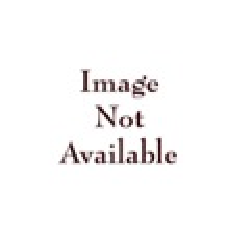
\includegraphics{noimage.eps}}\fi}
\def\szincludegraphics[#1]#2{%
      \if\showgraphics t{\includegraphics{#2}}%
      \else{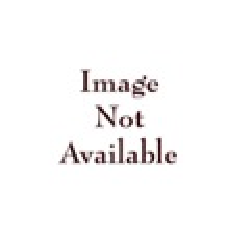
\includegraphics{noimage.eps}}\fi}

% kepler graphics
\def\pdffigtemplatex#1#2#3{%
\begin{figure}[htb]%
  \centering
  \myincludegraphics{\pdfp/#1}
  \caption{#3}
  \label{fig:#2}%
\end{figure}%
}
\def\pdfg#1#2#3{\if\showgraphics t{\pdffigtemplatex{#1}{#2}{#3}}\else{}\fi}


% tarski graphics
\def\pdffigtemplate#1#2#3{%
\begin{figure}[htb]%
  \centering
  \myincludegraphics{\pdf/#1}
  \caption{#3}
  \label{tarski:fig:#2}%
\end{figure}%
}
\def\pdffig#1#2#3{\if\showgraphics t{\pdffigtemplate{#1}{#2}{#3}}\else{}\fi}

%-%
% --Footnotes--
%-%
% http://help-csli.stanford.edu/tex/latex-footnotes.shtml
\long\def\symbolfootnote[#1]#2{\begingroup%
\def\thefootnote{\ensuremath{\fnsymbol{footnote}}}\footnote[#1]{#2}\endgroup}

%-%
% --Special Formatting--
%-%
% http://en.wikibooks.org/wiki/LaTeX/Formatting#List_Structures
\renewcommand{\labelitemii}{$\star$}


%-%
% --Indexing, References, Citations--
%-%
\def\indy#1#2{\index{index/#1}{#2}}

%-%
% --Proof Display--
%-%
% set with \displayallproof in flag_fly. If f, then proofs are swallowed.
%% "proved" environment. toggle with \displayallproof
%
\def\hide#1{}
\def\swallowed{\relax}
\def\swallow#1\swallowed{}
\newenvironment{iproved}{}{}
\newenvironment{proved}{\resetproved\begin{iproved}}{\end{iproved}}
\def\hideproof{\renewenvironment{iproved}{%
   \centerline{\it -- Proof Proofed --}
  \renewenvironment{itemize}{}{}
  \renewenvironment{enumerate}{}{}
  \def\item{\relax}
  \catcode13=12
  \swallow
}{}}
\def\showproof{\renewenvironment{iproved}{\begin{proof}}{\end{proof}}}
\def\resetproved{\if\displayallproof t\showproof\else\hideproof\fi}



%-%
% --Debugging Information--
%-%
\def\uf#1{{\par\narrower\it #1}} % unfinished manuscript
%% verbose:
\def\rating#1{\if\displayrating t{{\textsc {[rating={\ensuremath {#1}}].\ }}}\else{}\fi}
\def\oldrating#1{\if\displayrating t{{\textsc {[former rating={\ensuremath {#1}}].\ }}}\else{}\fi}
\def\formal#1{\if\verbose t{{\tt [formal: #1].\ }}\else{}\fi}
\def\formalauthor#1{\if\verbose t{{\tt [formal proof by: #1].\ }}\else{}\fi}
\def\footformal#1{\if\verbose t{\footnote{\formal{#1}}}\else{}\fi}
\def\usage#1{\if\verbose t{\symbolfootnote[1]{#1}}\else{}\fi}
\def\move#1#2{\begin{#1} See \ref{#2}.\end{#1}}
\def\FIXX#1{\if\verbose t{\footnote{\tt [#1]}}\else{}\fi}
\def\page#1#2{#2 {\it [dcgp.#1]}}
% first entry Lemma or Sec of DCG, second entry page.
\def\dcg#1#2{{\if\verbose t{{\tt{[DCG-#1]}}\indy{References}{ZC{#2 #1}@{DCG-#1}|page{#2}}}\else{}\fi}}
\def\tlabel#1{\label{#1}\if\verbose t{{\tt [#1].\ }%
   \indy{References}{#1|itt}}\else{}\fi}
\def\ifverbose#1{\if\verbose t{{#1}}\else{}\fi}




%% Indexing
\def\refXX{0} % for unknown links.
\def\showref#1{\ref{#1}{\tt[#1]}\indy{References}{#1}}
\def\oldlabel#1{\label{x-#1}}

\def\tref#1{\ref{#1}\indy{References}{#1}}
\def\itt#1{{\bf #1}}
\def\guid#1{{\tt[#1].\ }\indy{References}{ZA{#1}@{#1}|itt}}
% textsc
\def\calc#1{{\textsc{calc-#1}}\indy{Interval}{{#1}@{#1}}}
\def\newcalc#1{{\textsc{newcalc-#1}}\indy{Interval}{{#1}@{#1 (new XX)}}}
\def\assembly#1{{\textsc{assembly-#1}}\indy{References}{ZD{#1}@{#1}}}
%\def\conseq#1{{\textsc{conseq-#1}}}

%% 


%% Tarski indexing. Write summary data to external file "\mywrite",
% which is generated in tarski.tex
% Need to extend cs character set.  Use this only within a block.
\def\setcat{
\catcode`\-=11
\catcode`\.=11
\catcode`\:=11
\catcode`\0=11
\catcode`\1=11
\catcode`\2=11
\catcode`\3=11
\catcode`\4=11
\catcode`\5=11
\catcode`\6=11
\catcode`\7=11
\catcode`\8=11
\catcode`\9=11
}
\def\tarfe#1#2{{\foote{{\tt[L.E.G:#1]}~\csname #1-sum\endcsname%
  \expandafter\ifx \csname #1-guid\endcsname \relax [XX-BAD-IDENTIFIER]\else{}\fi
  }
  {\csname #1-guid\endcsname{#2}}}}
\def\tarf#1{\tarfe{#1}{}}
\def\tarfE#1{\tarfe{EE}{-\csname #1\endcsname}}
% control sequences will contain [-.0-9:] \catcode`\-=11, etc.
\newtoks\mysummary
\newtoks\myguid
\newtoks\myname
\def\separator{\if\tarskipagesep t{\clearpage}\else%
  \smallskip\hrule height 0.5pt depth 0pt width 60pt\bigskip\fi}
\def\identity#1{#1}
\def\foote#1#2{\footnote{#1~{\it (#2)}}}
\def\marker#1#2{\par\hangafter1\hangindent=1em\noindent{\bf #1:}\quad #2}
\def\name#1{\marker{Name}{#1}\myname={#1}
  \write\myhtml{  "#1", //name}
}
\def\summary#1{\marker{Summary}#1\mysummary={#1}
  % cleanse control sequences for html
  \if\tarskistrip t{
  \def\sqr{sqrt}
  \def\sqrt{sqrt}
  \def\op{\identity}
  \def\epsilon{epsilon}
  \def\Delta{Delta}
  \def\ups{upsilon}
  \def\beta{beta}
  \def\rho{rho}
  \def\CalE{E}
  \def\chi{chi}
  \def\eta{eta}
  \write\myhtml{  "#1", // summary}
  }
  \else\relax\fi
}
\def\guid#1{\if\tarskidump f{{\tt [#1]}}\else{\marker{ID}#1
   \indy{guid}{#1}
   \immediate\write\mywrite{\global\expandafter\def\csname \the\myname-sum \endcsname{\the\mysummary}}
   \immediate\write\mywrite{\global\expandafter\def\csname \the\myname-guid \endcsname{#1}}
   \immediate\write\myhtml{  "#1" // guid}}%
   \fi
}
\def\tag#1{\marker{Tags}#1
   \immediate\write\myhtml{  "#1", // tag}
}
%\def\rating#1{\marker{Rating}#1
%   \write\myhtml{  <rating>#1</rating>}
%}
\newenvironment{tarski}{%
\write\myhtml{new Tarski(}
%\def\name   {\marker{Name}}
%\def\summary{\marker{Summary}}
%\def\tag    {\marker{Tags}}
\def\rating {\marker{Rating}}
\def\hol{\marker{HOL-Light}}
%\def\guid   {\marker{ID}}
\def\tlabel{\label}
}{\separator\immediate\write\myhtml{),}
}
\newenvironment{tarskidata}{\write\myhtml{var tarskis=[}}
{
\immediate\write\myhtml{];}
}
%% tarski indexing
%\def\tarf#1{\footnote{{\tt geom-#1~\ref{#1}}\indy{ZA{#1}@{#1}}}}




%-%
% --Symbols--
%-%
% norm
\def\|{{\hskip0.1em|\hskip-0.15em|\hskip0.1em}}
\def\mid{\ :\ }
\def\norm#1#2{\|#1 - #2\|}
\def\normo#1{{\|#1\|}}
\def\sland{\ \land\ }
% Sam's
\def\myscorept{\text{ \sl pt}}
\def\qrtet{{quasi-regular tetrahedron}}
\def\qrtets{{quasi-regular tetrahedrons}}
\def\tomcite{{}}
\DeclareMathOperator{\myscore}{\sigma}
 \DeclareMathOperator{\gma}{gma}
 \DeclareMathOperator{\score}{\sigma}
 \DeclareMathOperator{\sol}{sol}
 \DeclareMathOperator{\dih}{dih}
\newtheorem{calcf}{Calculation}[subsection]

% mathcal
\def\CalB{{\mathcal B}}
\def\CalC{{\mathcal C}}
\def\CalD{{\mathcal D}}
\def\CalE{{\mathcal E}}
\def\FF{{\mathcal F}}
\def\CalF{{\mathcal F}}
\def\CalQ{{\mathcal Q}}
%\def\CalW{{\mathcal W}}
\def\CalR{{\mathcal R}}
\def\CalS{{\mathcal S}}
\def\CalV{{\mathcal V}}
\def\T{{\mathcal T}}
\def\Q{{\mathcal Q}}


% brackets
\def\leftopen{]}
\def\leftclosed{[}
\def\rightopen{[}
\def\rightclosed{]}

%% obsolete
\def\leftb{[}
\def\rightb{]}

% squiqqly relations
\def\seq{\approx}
\def\sle{\preceq}
\def\sge{\succeq}
\def\slt{\prec}
\def\sgt{\succ}

% mathbb
\def\R{{\mathbb R}}
\def\N{{\mathbb N}}
\newcommand{\ring}[1]{\mathbb{#1}}
\def\A{{\mathbf A}}
\def\Rp{\ring{R}^{3\,\prime}}

% operatorname
\def\op#1{{\operatorname{#1}}}
\def\optt#1{{\operatorname{{\texttt{#1}}}}}

\def\opat{\op{@}}
\def\atn{\op{arctan\ensuremath{_2}}}
\def\azim{\op{azim}}
\def\sol{\operatorname{sol}}
\def\vol{\op{vol}}
\def\quo{\operatorname{quo}}
\def\anc{\operatorname{anc}}
\def\cro{\operatorname{crown}}
%\def\vor{\operatorname{vor}}
%\def\svor{\operatorname{svor}}
\def\sign{\operatorname{sign}}
\def\octavor{\operatorname{octavor}}
\def\dih{\operatorname{dih}}
\def\Adih{\operatorname{Adih}}
\def\arc{\operatorname{arc}}
\def\cosarc{\operatorname{cosarc}}
\def\rad{\operatorname{rad}}
\def\gap{\operatorname{gap}}
\def\sc{{\operatorname{sc}}}
\def\geom{{\operatorname{g}}}
\def\anal{{\operatorname{an}}}
\def\PM{\operatorname{PM}}
\def\bool{\operatorname{bool}}
\def\true{\op{true}}
\def\false{\op{false}}
\def\flat{\operatorname{flat}}
\def\tangle#1{\langle #1\rangle}
\def\ceil#1{\lceil #1\rceil}
\def\floor#1{\lfloor #1\rfloor}
\def\ups{\upsilonup} % Needs txfonts; else use \upsilon
\def\orgn{\varthetaup} % center of packing
%\def\comp#1{\llbracket #1 \rrbracket}
\def\comp#1{[#1]}
\def\Wdart{W_{\text{dart}}}
\def\Wedge{W_{\text{edge}}}
\def\cell{\operatorname{cell}}

\def\SA{A}
\def\SB{B}
\def\SC{C}
\def\SD{D}
\def\SE{E}
\def\del{\partial}
\def\doct{\delta_{oct}}
\def\dtet{\delta_{tet}}
\def\pt{\hbox{\it pt}}
\def\hm{{h_0}} % 1.26
%\def\Vol{\hbox{vol}}
\def\scoregoal{8\,\pt}
\def\maxpi{\pi_{\max}}
\def\tausc{{\tau\!\operatorname{sc}}}
\def\piF{{\pi_F}}
\def\xiG{\xi_\Gamma}
\def\piG{\pi_\Gamma}
\def\xiV{\xi_V}
\def\xik{\xi_\kappa}
\def\xikG{\xi_{\kappa,\Gamma}}
\def\piV{\pi_V}
\def\tauLP{{\tau_{\hbox{\twrm LP}}}}
\def\DLP{\operatorname{D}_{\hbox{\twrm LP}}}
\def\ZLP{\operatorname{Z}_{\hbox{\twrm LP}}}
\def\tlp{\tau_{\hbox{\twrm LP}}}  % 2 args (p,q) tri, quad
\def\sLP{\sigma_{\hbox{\twrm LP}}}  % 2 args (p,q) tri, quad
\def\squander{(4\pi\zeta-8)\,\pt}
\def\trgt{\operatorname{\it{target}}}
\def\tildeF{{\hbox{$\tilde F$}}}
\def\zloop{{z}_{loop}}
\def\dloop{{\delta}_{loop}}
\def\sqr{\sqrt}
\def\tildeV{V^{\CalS}}
%\def\BigD{\Delta}
%\def\bigd{\Delta^0}
\def\FCinner{\op{FC}_{\text{inner}}}
\def\FC{\op{FC}}
\def\FCR{\op{FCR}}
\def\rogFC{\op{rog}^0_{\text{FC}}}
\def\chino{\chi_0}

\def\x#1{\op{\bf c}{#1}}  % marks context \x(p,r).
\def\xs#1{\op{\bf sc}{#1}}  % marks special context \x(p,r,s).
\def\xtazimlt{\x{(3,1: \op{azim}(\op{gap}) <\pi)}}
\def\xtazimge{\x{(3,1: \op{azim}(\op{gap}) \ge \pi)}}
\def\xfgap{\x{(4,1:\op{gap})}}
\def\y#1{\op{\bf ep}{#1}}  % marks edge parameters \y(n,k).
\def\pqr#1{#1} % marks type (p,q,r).
%\def\pqr#1{\op{\bf typ}{#1}} % marks type (p,q,r).

%% HYPERMAP macros:
% avoid e for both hypermap edge and edge {v,w}
\def\e{\varepsilonup}
\def\ocirc{}



%% FORMULATION macros:
\def\lam{\lambda}
\def\Lam{\Lambda}
\def\bl{{\underline{\lam}}}
\def\bm{{\underline{\mu}}}
\def\angle#1#2#3{{\op{angle}(#1,{#2,#3})}}


\def\card{\op{card}}

% accent used in India citation in Overview.
\def\=#1{\accent"16 #1}
\def\i{I}
%\def\={\relax}



%% Enclosed CALE control sequences:
\expandafter\def\csname 2t0-doesnt-pass-through\endcsname{01}
\expandafter\def\csname E1453\endcsname{02}   
\expandafter\def\csname dcg-p89\endcsname{03}   
\expandafter\def\csname enclosed-v\endcsname{04}   
\expandafter\def\csname 277\endcsname{05}   
\expandafter\def\csname 245\endcsname{06}   
\expandafter\def\csname 245bis\endcsname{07}   
\expandafter\def\csname node\endcsname{08}   
\expandafter\def\csname E:part4:1\endcsname{09}   
\expandafter\def\csname E:part4:2\endcsname{10}   
\expandafter\def\csname E:part4:3\endcsname{11}   
\expandafter\def\csname E:part4:4\endcsname{12}   
\expandafter\def\csname E:part4:5\endcsname{13}   
\expandafter\def\csname E:part4:6\endcsname{14}   
\expandafter\def\csname E:part4:7\endcsname{15}   
\expandafter\def\csname E:part4:8\endcsname{16}   
\expandafter\def\csname E:part4:9\endcsname{17}   
\expandafter\def\csname E:part4:10\endcsname{18}   
\expandafter\def\csname dcg-p142\endcsname{19}   
\expandafter\def\csname convex-quad\endcsname{20}   
\expandafter\def\csname last:E\endcsname{21}
\expandafter\def\csname rem2.7\endcsname{22}     
\expandafter\def\csname pass-anchor\endcsname{23}

%% 
 
 
 
 
 
 
 

%\def\indy#1#2{\relax}

%%%%%%%%%%%%%%%%%%%%%%%%%%%%%%%%%%

\begin{document}

\title{Math 3600: Lectures on the Langlands-Tunnell theorem}
\author{Thomas C. Hales}
%\institute{\hbox{ }}
\maketitle


    \tableofcontents


%\begin{abstract}  
%\end{abstract}

%%%%%%%%%%%%%%%%%%%%%%


\parindent=0pt
\parskip=\baselineskip
\def\seg{~~~}
\def\text{\hbox}

These are lectures from a course on the Langlands-Tunnell theorem, during
the Spring 2012 semester in the math department at the University of Pittsburgh.%
\footnote{\svninfo}
Every effort has been made to keep the prerequisites to a minimum.
For background in Algebra, we use Knapp's Basic Algebra \cite{knapp-basic}.
For algebraic number theory and class field theory, 
we use Milne's notes 
\cite{ANT}, \cite{CFT}.  For local Langlands, we use \cite{bushnell-henniart}.
All of these books go to significant lengths to give detailed and self-contained 
proofs.

\section{Fermat's Last Theorem}

This lecture was delivered on Monday, January 4, 2012.

Fermat's Last Theorem \cite{DDT} states the equation
\[
a^n + b^n = c^n,
\]
has no solution in the integers when $n>2$ and $abc\ne 0$.  There are
infinitely many solutions when $n=2$:
\[
3^2 + 4^2 = 5^2,\quad 5^2 + 12^2 = 13^2, \ldots
\]
Fermat himself did not write down a proof, and it eventually became
the most famous problem in the history of mathematics.  There have
been many attempts through the centuries.  Over 1000 false proofs of
the result were published between 1908 and 1912.  It was solved by
A. Wiles, with some assistance from R. Taylor.

If there is a proof for exponent $n$ and if $N = n r$, then
\[
(a^r)^n + (b^r)^n = (c^r)^n,
\]
settles the exponent $N$ as well.  Any exponent $N\ge3$, is divisible
by $4$, divisible by $3$, or divisible by a prime $n\ge 5$.  Fermat
gave a proof when the exponent $n$ is $4$.  Euler gave a proof for
exponent $3$.  The case that remains is a prime exponent $n\ge 5$.  We
assume $n\ge5$ in what follows.

Frey suggested that we argue by contradiction.  Let
$(A,B,C)=(a^n,b^n,c^n)$ be a solution: $A+B=C$, with $ABC\ne
0$. Consider the curve
\[
y^2 = x (x - A) (x + B).
\]
The cubic has distinct roots, exactly when $0$, $-A$ and $B$ are
distinct, which occurs if and only if $abc\ne 0$.  By factoring out
common powers of $2$, we may assume that at least one of $A$, $B$, $C$
is odd.  By considering parity, at least one of them is even.
Reordering, we may assume that $A$ is odd and $B$ is even.  In fact,
$B=b^n$, with $n\ge 5$, is divisible by $32$.


The Frey curve is an elliptic curve.  What was Frey's motivation?  Who
knows! Perhaps it was an act of desperation when nothing else seemed
to work. At least elliptic curves have been studied very extensively.

The set of complex solutions, including a point at infinity is a
topological torus, a product of two circles.  The set of points of
order $3$ is $\ring{F}_3^2$, a two dimensional vector space over the
field with three elements.  Each automorphism of the group is
necessarily linear, hence an invertible linear transformation of
$\ring{F}^2_3$.  All such automorphisms form a group
$GL(2,\ring{F}_3)$.

The group law can be expressed algebraically: there is a collection of
polynomials\footnote{To be entirely correct, we should take the
  polynomials to be homogeneous polynomials in the variables
  $x_i,y_i,z_i$, for $i=1,2,3$, where $[x_i:y_i:z_i]$ gives the
  homogeneous coordinates of the points in projective space.}  with
rational coefficients in six variables such that
$(x_1,y_1),(x_2,y_2),(x_3,y_3)$ is a simultaneous zero of the
polynomials if and only if $(x_1,y_1)$, $(x_2,y_2)$, and $(x_3,y_3)$
are points on the elliptic curve and $(x_3,y_3)$ is the sum of
$(x_1,y_1)$ and $(x_2,y)$.  By convention, the identity element is
taken to be point at infinity.  It is known that the set
\[
E[3]= \{(x,y) \in \ring{C}^2\mid y^2 = x (x-A) (x+B), 
\quad (x,y) \text{ has order } 3\}\cup \{\infty\}
\]
is the set of roots of polynomials with rational coefficients,
together with the point at infinity.  The set of coefficients $(x,y)$
of these nine points lie in a finite Galois extension $K$ of
$\ring{Q}$.

If $\sigma$ is an automorphism of $K/\ring{Q}$, then it permutes the
set $E[3]=\ring{F}_3^2$ and it respects the group law, hence is
expressed as an element of $GL(2,\ring{F}_3)$.  In fact, we obtain a
homomorphism
\[
\phi_1 : \op{Gal}(K/\ring{Q}) \to GL(2,\ring{F}_3).
\]
Part of Wiles's proof shows that we may assume without loss of
generality that this representation is irreducible; that is, there is
no $1$-dimensional vector space that is stable under
$\op{Gal}(K/\ring{Q})$.

The group $GL(2,\ring{F}_q)$ is a finite group of order
$(q^2-1)(q^2-q)$.  When $q=3$, we get a group of order $48$.  For a
moment, view $GL(2,\ring{F}_3)$ as an abstract group.  It is known
to have a $2$-dimensional faithful representation,
\[
\phi_2 : GL(2,\ring{F}_3) \to GL(2,\ring{C}).
\]
The composite of $\phi_1$ and $\phi_2$ gives a homomorphism
\[
\op{Gal}(K/\ring{Q}) \to GL(2,\ring{C}).
\]

It is the aim of this course to understand this homomorphism.  The
Langlands-Tunnell theorem implies that the strong Artin conjecture
holds for this homomorphism.  We will have much more to say about this
later.


\newpage
\section{Finite subgroups of $GL(2,\ring{C})$}

Lecture delivered Friday January 6, 2012.


Basic facts about the representations of finite groups can be reviewed
in \cite[p.~326, Sec. VII.4]{knapp-basic}; Facts about symmetric and
hermitian 
forms are found at \cite[p.~250,~Sec.~VI.2,~VI.4]{knapp-basic}.

If $V$ is a vector space over a field $F$, we write $GL(V)$ (the
general linear group) for the group of invertible linear maps $g:V\to
V$.  If $V=F^n$ for some field $F$, we write $GL(n,F)$ for
$GL(n,F^n)$.  It is identified with the set of $n$ by $n$ matrices
with coefficients in $F$ with nonzero determinant.  More generally, if
$R$ is a commutative ring with $1$, we write $GL(n,R)$ for the group
of $n$ by $n$ matrices with coefficients in $R$ whose determinant is a
unit in $R$.

If $V$ is an $R$ module, where $R$ is a commutative ring with $1$, 
we write $\op{End}_R(V)$ for the ring of $R$-module endomorphisms of $V$.

A \newterm{representation} is a homomorphism $\phi$ from a group $G$
into $GL(V)$ for some vector space $V$.  We write $(\phi,V)$ for the
representation, which we abbreviate at times to $\phi$ or $V$.  
The representation is \newterm{reducible} if there is
a subspace $W\ne 0,V$ of $V$ such that $\phi(g)w\in W$ for all $g\in
G$ and $w\in W$.  It is \newterm{irreducible} if it is not reducible.
The representation is \newterm{faithful} if the kernel of $\phi$ is
$1$.

We let $U(n)$ be the group of $n$ by $n$ unitary matrices:
\[
U(n) = \{ g \in GL(n,\ring{C})  \mid \t{\bar g} g = I\},
\]
where the $t$ marks transpose, $\bar g$ is the coefficient-wise
conjugate of $g$, and $I=I_n$ is the identity matrix.  We let $O(n,F)$
be the group of $n$ by $n$ orthogonal matrices:
\[
O(n,F) = \{ g \in GL(n,F) \mid \t{g} g = I\},
\]
We write $SL(n,F)$, $SL(V)$, $SU(n)$, and $SO(n,F)$ for the subgroups
of $GL(n,F)$, $GL(V)$, $U(n)$, $O(n,F)$ respectively of those linear
transformations with determinant $1$.  Note that if a matrix $g$ is orthogonal,
then $\det(g)^2 = \det(\t{g}g) = \det{I} = I$, so that its determinant is $\pm 1$.

For example $SU(2)$ is given by the set of matrices with complex entries satisfying
\[
\begin{pmatrix}{\bar a} & {\bar c} \\ \bar b & \bar d\end{pmatrix} = 
\begin{pmatrix}d & - b\\ -c & a \end{pmatrix},\quad ad - bc = 1;
\]
or equivalently, complex matrices of the form
\[
\begin{pmatrix}a & b\\ -\bar b & \bar a\end{pmatrix},\quad |a|^2 + |b|^2 = 1.
\]
As a topological space, the set $SU(2)$ is homeomorphic to
 the $3$-sphere 
$$\{(a,b)\in \ring{C}^2\mid |a|^2 + |b|^2 = 1\}.$$


\begin{lemma} If $G$ is any finite subgroup of $GL(2,\ring{C})$, then it is
conjugate to a subgroup of $U(2)$.
\end{lemma}

\begin{proof} Fix any positive definite hermitian form $v,w\mapsto \langle v,w\rangle $ on $\ring{C}^2$;
say 
\[\langle (z_1,z_2),(w_1,w_2)\rangle  = z_1 \bar w_1 + z_2 \bar w_2\]
Let $\langle v,w\rangle_1 = \sum_{g\in G} \langle v,w\rangle$.  This is again a positive definite
hermitian form.    Then $G$ preserves $\langle\cdot,\cdot\rangle_1$ and with respect 
to an orthonormal basis  of $\langle\cdot,\cdot\rangle_1$, the matrices representing $G$ are unitary.
\end{proof}

We define a representation $\phi$ of $U(2)$ in $GL(3,\ring{R})$ by the action of $U(2)$ on the real $3$-dimensional
 vector space $H$
of $2$ by $2$ Hermitian matrices.
\[
H = \{ X \mid \t{\bar X} = X,\quad \op{trace}(X)=0\}, and 
\]
  \[
   \phi(g) X = {g} X g^{-1} \in H, \quad X\in H.
  \]
We claim that the image $\phi(U(2))$ is conjugate to a subgroup of  $SO(3,\ring{R})$.
First we check that the image is conjugate to a subgroup of $O(3,\ring{R})$.  We define an inner product
on $H$ by  $X,Y\mapsto \op{trace}(XY)$.  It is symmetric by a basic property of the trace.  Note that 
\[
\bar {\op{trace}(XY)} = \op{trace}(\bar X \bar Y) = \op{trace}(\t{X}\t{Y}) = \op{trace}(\t{(YX)}) = \op{trace}(XY),
\]
so that the inner product takes real values.
Also, if we take a general element of $H$ of the form
\[
X = \begin{pmatrix} a & b + i c \\ b - i c & a\end{pmatrix},
\]
we compute $\op{trace}(X^2) = 2 (a^2 + b^2 + c^2)$.  This gives that the inner product is positive definite.  We may
pick an orthonormal basis for this inner product.  With respect to this basis, the image $\phi(U(2))$
is represented by orthogonal matrices.

Next we check that the image consists of matrices of determinant $1$.
Recall that the determinant of an orthogonal matrix is $\pm 1$.
The set $\det\phi(SU(2))$ is the continuous image of the $3$-sphere, which is a connected topological space.  The
image contains $1$ (image of the identity).  Hence the image of $SU(2)$ under $\det\phi$ is $1$.  Similarly,
the image of the set of scalar matrices in $U(2)$ is the continuous image of a circle, which is again a connected
topological space.  Since every unitary matrix is a product of a scalar matrix with a special unitary matrix,
the result follows.

\begin{lemma} Every matrix $g\in SO(3,\ring{R})$ has  eigenvalue $1$.
\end{lemma}

\begin{proof}
\[
\det (g-I) = \det(\t{g}-I) = \det(g^{-1}-I) = \det(g^{-1})\det(I - g) = 
\det(-I)\det(g - I) = -\det(g-I).
\]
So $\det(g-I)=0$, and $g-I$ is singular.
\end{proof}

\begin{theorem}
Let $G$ be a finite subgroup of $SO(3,\ring{R})$.  Then $G$ is cyclic, dihedral,
or the group of symmetries of a Platonic solid.
\end{theorem}

There are five Platonic solids: tetrahedron, octahedron, cube, dodecahedron, and icosahedron.
There are only three symmetry groups because the octahedron and cube have the same symmetry group,
and the dodecahedron and icosahedron have the same symmetry group.

\begin{proof}
\claim{If $1\ne g\in G$, then it has a eigenvalue $1$ with multiplicity $1$.}  Let $v$ be an eigenvector
of $g$ with eigenvalue $1$.  Then $g$ is a rotation about the line through the origin and $v$.  The other
two eigenvalues are $exp(\pm i \theta)$, where $\theta$ is the angle of rotation.  Hence another eigenvalue
is one if and only if the angle of rotation is $0$.

We call an eigenvector of $1\ne g\in G$, normalized to have length $1$, a pole of $g$.  let $P$ be the
set of all poles of all $1\ne g\in G$.  
The group $G$ acts on the set $P$: if $v\in P$ is a pole of $g$, then $h v$ is a pole of $h g h^{-1}\in G$.

Let $O_1,\ldots O_k$ be the orbits of $G$ in $P$, and let $r_i=\card(G_v)$, for $v\in O_i$,
where $G_v$ is the stabilizer of $v\in P$.
A basic property
of transitive group actions is that $O_i$ can be identified with the coset space $G/G_v$.
In particular, $\card(O_i) = n/r_i$, where $n=\card(G)$.

The set
\[
\{(g,v)\mid g\ne 1,\quad v \hbox{ is a pole of } g\}
\]
can be counted two ways: either grouping by the first coordinate, or by the second coordinate.
For every first coordinate there are two second coordinates.  Alternatively,
for every orbit $O_i$ and every second coordinate $v\in O_i$, there
are $r_i - 1$ first coordinates.  Counting both ways, we get
\[
2 (n-1) = \sum_{i=1}^k \card{(O_i)}\, (r_i - 1) =  \sum \frac{n}{r_i}(r_i-1),
\]
or after dividing by $n$:
\[
2 (1 - 1/n) = \sum_{i=1}^k (1-1/r_i).
\]
Each $r_i$ is the order of a nontrivial group, so $r_i\ge2$.
This gives
\[
2 > 2 (1-1/n) =\sum_{i=1}^k (1-1/r_i) \ge k/2.
\]
This implies $k\le 3$.  
In the other direction
\[
1 \le 2(1-1/n) = \sum_{i=1}^k (1-1/r_i) < \sum_{i=1}^k 1 \le k.
\]
This implies $2\le k$.

We consider each case $k=2,3$ in turn.

If $k=2$, then the equality can be written
\[
2/n = 1/r_1 + 1/r_2 \ge 1/n + 1/n.
\]
This implies $n=r_1 = r_2$ so that the order of the stabilizer of a
pole $v\in O_1$ is the order of the group.  This forces $G$ to be
cyclic, consisting of rotations about the line through $v$.

If $k=3$, the equality takes the form
\[
1< 1 + 2/n = 1/r_1 + 1/r_2 + 1/r_3.
\]
We make an exhaustive lexicographical search over all triples
$(r_1,r_2,r_3)$ that satisfy
\[
1 < 1/r_1 + 1/r_2 + 1/r_3, \hbox{ and } r_1 \le r_2 \le r_3,
\]
where $r_i \in \{2,3,\ldots\}$.
The only solutions are 
\[
\{ (2,2,r)\mid r\ge 2\} \cup \{(2,3,3),(2,3,4),(2,3,5)\}.
\]
The order $n$ of $G$ in these respective cases is $2r$, $12$, $24$,
and $60$.  From the explicit information about orbits and stabilizers
thus obtained, an easy exercise shows that these cases correspond to
the dihedral, tetrahedral, octahedral, and icosahedral symmetry groups
respectively.  For example, in the first case, the set $O_1$ is the
set of vertices of a regular $r$-gon. In the other cases, the three
orbits $O_1$, $O_2$, $O_3$ are (the projections to the unit sphere of)
the edge midpoints, vertices, and face centers of the Platonic
solid (or its dual).
\end{proof}

The structure of the groups of rotations of the Platonic solids are well-known.
Every symmetry of the tetrahedron acts on its set of four vertices, giving
an embedding of the group into $S_4$.  Elements of $SO(3,\ring{R})$ act as
even permutations, so that the group is isomorphic to $A_4$.

The group of the cube/octahedron acts as permutations of the four lines passing
from vertex to opposite vertex of a cube.  This injects the octahedral group
into $S_4$.  Since they have the same order, this is an isomorphism.

The $20$ vertices of the dodecahedron can be partitioned into $5$ sets of cardinality
four in such a way that each set is the set of vertices of a regular tetrahedron.
The group of the dodecahedron/icosahedron acts as a group of order $60$ 
on this set of five
regular tetrahedra.  This is a subgroup of index $2$ in $S_5$, which uniquely
characterizes  $A_5$.  Thus, the icosahedral group is isomorphic to $A_5$.

We have noted that $GL(2,\ring{F}_3)$ is isomorphic to a subgroup of
$GL(2,\ring{C})$.  Its image in $SO(3,\ring{R})$ is octahedral.  Let
$Z$ be the subgroup (of order $2$) consisting of scalar matrices.  We
show that $GL(2,\ring{F}_3)/Z$ is $S_4$ directly as follows.  Let
$\ring{P}^1(\ring{F}_3)$ be the projective line over the field with
three elements.  Concretely, the projective line over a field $F$ is
given by the set of equivalence classes of
\[
X(F)=F^2 \setminus \{(0,0)\},
\]
under the equivalence relation $(z_1,z_2)\sim (t z_1,t z_2)$, for
$t\in F^\times$.  When $F=\ring{F}_q$, the cardinality of $X(F)$ is
$q^2-1$, and each equivalence class has $q-1$ elements, so that
$\ring{P}^1(\ring{F}_q)$ has cardinality $(q^2-1)/(q-1)=(q+1)$.  The
group $GL(2,\ring{F}_q)$ acts on $\ring{P}^1(\ring{F}_q)$ through the
usual matrix multiplication on $X(F)$.  When $q=3$, the projective
line has cardinality $4$, the subgroup $Z$ acts trivially, and this
action gives an isomorphism of $GL(2,\ring{F}_3)/Z$ with $S_4$.


\newpage
\section{Cyclic and Dihedral subgroups}

Lecture Wednesday, January 11, 2012.


Let $G$ be a finite group and $V$ a vector space over a field $F$.  
Every representation $(\phi,V)$ of $G$
is a module of the group algebra $F[G]$ by the rule 
\[
[g].v = \phi(g)v, \text{ where } [g]\in F[G].
\]
Conversely, if $V$ is an $F[G]$ module, the same rule read in the opposite
direction defines a representation
\[
\phi:G\to GL(V).
\]
Thus, we may switch back and forth between the language of representation
theory and the language of modules, sometimes referring to $(\phi,V)$ as
a module.

Let $\phi:H\to GL(V)$ be a representation of a subgroup $H$ of a
finite group $G$, where $V$ is a vector space over a field $F$.  There
is a universal way to construct from $(\phi,V)$ a representation $\op{Ind}_H^G\phi$ of
$G$, called induction.\footnote{We write $\op{Ind}_H^G V$ for the vector space on
which it acts, or sometimes $\op{Ind}_H^G (\phi,V)$ for the ensemble.}  
It may be described as a tensor product
\[
\op{Ind}_H^G(V) = F[G]\otimes_{F[H]} V,
\]
where $F[\cdot]$ denotes the group algebra.  The group $G$ acts
naturally on the vector space $F[G]$ and hence on the tensor product.

\begin{exercise}
If $S$ is a set of representatives of $G/H$, then $\op{Ind}_H^G(V)$
has dimension $\card(G/H)\dim_F(V)$, and has basis $[s]\otimes v_i$,
for $s\in S$ and $v_1,\ldots $ a basis of $V$.
\end{exercise}

In categorical terms, induction is the left adjoint of the restriction functor
from the category of  $F[G]$-modules to the category of  $F[H]$-modules.
We leave this as an exercise to the reader.  The adjointness is expressed as a 
natural bijection
\begin{equation}\label{eqn:adjoint}
\op{Hom}_{F[G]}(Ind_H^G V,W) = \op{Hom}_{F[H]}(V,\op{Res}_H W),
\end{equation}
where $\op{Res}_H W$ is the restriction of the $F[G]$-module $W$ to $F[H]$.

Two representations $\phi_1:G\to GL(V)$, $\phi_1:G\to GL(W)$ are
\newterm{equivalent} if $V$ and $W$ are isomorphic as $F[G]$-modules.

\begin{theorem}
  Let $\phi:G\to GL(2,\ring{C})$ be an irreducible $2$-dimensional
  representation of a finite group $G$.  Assume that the image of $G$
  in $SO(3,\ring{R})$ is cyclic or dihedral.  Then exists a subgroup
  $H$ of $G$ of index $2$ and a $1$-dimensional representation
  $\theta$ of $H$, such that $\phi$ is equivalent to
  $\op{Ind}_H^G\theta$.
\end{theorem}

In an earlier lecture, we constructed a homomorphism $U(2)\to
SO(3,\ring{R})$ by having $U(2)$ act on the three dimensional real
vector space $H$ of Hermitian matrices in $\op{End}(\ring{C}^2)$ with
trace zero.  The complexification
$sl(2,\ring{C})=\ring{C}\otimes_{\ring{R}} H$ is the three dimensional
complex vector space of all $2$ by $2$
matrices of trace zero.  Over the complex vector space, the
homomorphism $U(2)\to SO(3,\ring{R})$ extends to a homomorphism
$GL(2,\ring{C})\to GL(3,\ring{C})$.  The action is the same as before
\[
(g,X)\mapsto g X g^{-1},\quad X\in sl(2,\ring{C}).
\]
If $g = \begin{pmatrix} a& b\\ c & d\end{pmatrix}$, then the inverse
of $g$ is given by a well-known formula
\[
g^{-1} = \frac{1}{\det{g}}\begin{pmatrix} d & - b \\ -c & a\end{pmatrix} 
= \det g^{-1} J \t{g} J^{-1}, \quad
\hbox{ where } J = \begin{pmatrix} 0 & -1 \\ 1 &0 \end{pmatrix}
\]
Let $S$ be the $3$-dimensional complex vector space of all symmetric matrices in $\op{End}(\ring{C}^2)$.
We have a linear isomorphism $sl(2,\ring{C})\to S$, given by $X\mapsto X J$:
\[
\begin{pmatrix} a& b\\c & -a\end{pmatrix} \begin{pmatrix} 0& -1 \\1 &0\end{pmatrix} = 
\begin{pmatrix} b & -a \\ -a & -c \end{pmatrix}
\]
If we carry the action of $GL(2,\ring{C})$ on $sl(2,\ring{C})$
over to $S$ by this isomorphism, we get by a simple calculation
\[
(g,A) \mapsto \det(g)^{-1} g A \t{g},\quad A \in S.
\]

We are ready to give a proof of the theorem.

\begin{proof} Identify (a factor group of) $G$ with a subgroup of
  $U(2)$ by means of $\phi$.  A cyclic or dihedral subgroup of
  $SO(3,\ring{R})$ has a line that is stable under the subgroup (that
  is, a common eigenvector). Using our explicit description of the
  three-dimensional vector space as Hermition matrices, the stable
  line corresponds to a non-zero Hermitian matrix $X$ such that
\[
g X g^{-1} = \lambda(g) X,
\]
for all $g\in G$ for some scalar $\lambda(g)$, depending on $g$.
The determinant of a general non-zero hermition matrix of trace $0$ is non-zero:
\[
\det\begin{pmatrix} a & b + i c\\ b - i c & -a\end{pmatrix} = -a^2 - b^2 - c^2 \ne 0.
\]
The symmetric matrix $A = X J$ also has non-zero determinant.  In
terms of the action of $G$ on symmetric matrices, the stable line
condition becomes
\[
g A \t{g} = \lambda(g)\det(g) A.
\]
(All such $g$ form a group of orthogonal similitudes.)  We define an
inner product on row vectors $\ring{C}^2$ by $v,w\mapsto \langle
v,w\rangle = v A \t{w}$.  Since $\det A\ne 0$, it is non-degenerate.
All non-degenerate inner products on $\ring{C}^2$ are equivalent by
basic facts of quadratic forms over $\ring{C}$ (see \cite{knapp-basic}).  Hence there is a
basis of $\ring{C}^2$ such that $A$ takes the form
\[
A_1 = \begin{pmatrix} 0 & 1 \\ 1 & 0\end{pmatrix}
\]
The stable line condition becomes
\begin{equation}
g A_1 \t{g}=\begin{pmatrix} a & b \\ c & d\end{pmatrix} 
\begin{pmatrix} 0 & 1 \\ 1 & 0\end{pmatrix}
\begin{pmatrix} a & b \\ c & d\end{pmatrix} = 
\begin{pmatrix} 2 a b & * \\ * & 2 c d\end{pmatrix} =
\begin{pmatrix} 0 & * \\ * & 0\end{pmatrix} = \lambda(g)\det(g) A_1.
\end{equation}
Hence $ab=0$ and $cd=0$.  This forces $g$ to be diagonal $b=c=0$ or
antidiagonal $a=d=0$.  

Let $N(T)$ be the group 
\[
\{\begin{pmatrix} a & b \\ c & d\end{pmatrix} \in GL(2,\ring{C}) \mid
b = c =0 \quad \text{ or } a = d = 0\}.
\]
The diagonal group $T$ has index two in $N(T)$.
The nontrivial coset is represented by an  antidiagonal matrix.

If $G\subset T$, then $\phi$ is reducible,
contrary to assumption.  Hence the composite,
\[
G\to N(T)\to N(T)/T = \ring{Z}/2\ring{Z}
\]
is onto, and its kernel is a subgroup $H\subset T$ of index $2$ in $G$.
Let
$\theta_i:H\to GL(1,\ring{C})$, for $i=1,2$, be the diagonal entries
of $H$.  Let $w$ be a representative of the nontrivial coset of $H$ in
$G$.  Conjugation of $H$ by $w$ permutes its diagonal entries, so
$\theta_1(w h w^{-1}) = \theta_2(h)$ for $h\in H$.  If
$\theta_1=\theta_2$, then $H$ consists of scalars, and again we find
that $\phi$ is reducible.  Hence $\theta_1\ne\theta_2$.  A short
exercise based on the adjointness property (\ref{eqn:adjoint}) now
shows that $\op{Ind}_H^G\theta_1$ is irreducible and $\phi$ is
equivalent to $\op{Ind}_H^G\theta_1$ via the morphism of modules:
\[
1\in\op{Hom}_{F[H]}(\theta_1,\theta_1)=\op{Hom}_{F[H]}(\theta_1,\theta_1\oplus\theta_2)=
\op{Hom}_{F[H]}(\theta_1,\op{Res}_H\phi) = \op{Hom}_{F[G]}(\op{Ind}_H^G\theta_1,\phi).
\]
\end{proof}

\newpage
\section{Topological Groups}

In this section, we assume basic familiarity with point-set topology,
including connectedness, compactness, and so forth. 

A topological group is a group $G$, together with a topology on that
group, such that the maps
\[
\mu:G\times G\to G,\quad \iota:G\to G,
\]
are continuous, where $\mu$ and $\iota$ are multiplication and
inverse, respectively.  The topology on $G\times G$ is the product
topology.

Warning -- the word {\it closed} now has two meanings, a closed subset
in topology, and in the sense of a set being closed under
multiplication.  If in doubt, we probably intend the topological
meaning.

The notion of topological group is particularly fruitful; we should
consider {\it every} group as a topological group, falling back to the
discrete topology on $G$ if nothing else comes to mind.

(More generally, we may consider topological rings, topological
modules, and so forth, where each is defined as an algebraic
structure, together with a topology, for which all the algebraic
operations are continuous.)

There are many examples of topological groups $GL(n,F)$, $SL(n,F)$,
$SO(n,F)$, vector spaces over $F$, where $F=\ring{R}$ or $\ring{C}$.
Also, $U(n)$, $SU(n)$ are topological groups.  In all of these cases the
continuity of matrix multiplication is obvious, since each matrix
coefficient of the product is polynomial in the matrix coefficients of
the factors.  The continuity of of the matrix inverse for invertible
matrices follows from Cramer's rule \cite[Prop.~5.4]{knapp-basic} for
the inverse of $g\in GL(n,F)$:
\[
\det(g) g^{-1} = \text{  matrix of cofactors of } \t{g}.
\]
Cofactors are determinants, hence polynomial, hence continuous.

A finite group is a topological group in the discrete topology.

A topological group inherits notions from topology: it can be
discrete, connected, compact, locally compact, etc.

Let's proof a few simple facts about topological groups.  (Proofs are
generally easy in this branch of mathematics.)

\begin{lemma}
Let $L_g:G\to G$ be left translation in a topological group $L_g(h) = g h$.
Then $L_g$ is homeomorphism.  Similarly, right translation is a homeomorphism.
\end{lemma}

\begin{proof}
It is continuous, given as 
a composite of continuous maps $\{g\}\times G \to G\times G \to G$.
Its inverse $L_{g^{-1}}$ is also continuous.
\end{proof}

\begin{lemma}  The neighborhoods of $g\in G$ have the form $g U$ (or $Ug$),
where $U$ is a neighborhood of $e\in G$.
\end{lemma}

\begin{proof} $L_g$ is a homeomorphism.
\end{proof}

\begin{lemma} If $U$ is a neighborhood of $e\in G$, there is an open neighborhood  $V$ of $e$
such that $V= V^{-1}$ and $VV \subset U$.
\end{lemma}

\begin{proof} By the definition of the product topology, $\mu^{-1}(U)$ contains an open
neighborhood of $e$ of the from $W\times W$.  The open set $V = W\cap W^{-1}$ works.
\end{proof}

\begin{lemma} Let $G$ be a topological group and $H$ a closed subgroup.  Fix $g\ne H$.
Then there exists disjoint open sets $V_1,V_2$ such that $H\subset V_1$ and $gH\subset V_2$.
\end{lemma}

\begin{proof}  Let $U$ be the open set $G\setminus g H$.  Let $V$ be as in the
previous lemma.  Then $V_1 = VH$ and $V_2 = VgH$ works.  To check disjointness,
\[
v_1 g h_1 = v_2 h_2 \Longrightarrow U \owns v_1^{-1}v_2 = g h_1 h_2^{-1} \in g H.
\]
\end{proof}

\begin{lemma} if $\{e\}$ is closed, then $G$ is Hausdorff.
\end{lemma}

\begin{proof} Take $H = \{e\}$ in the previous lemma.
\end{proof}

If $X$ is any topological space and $\sim$ is any equivalence relation,
we let $X/\sim$ be the set of equivalence classes.  There is a canonical
projection $p:X\to X/\sim$.  We put the quotient topology on $X/\sim$:
a set $U$ is declared open if and only if $p^{-1}U$ is open.

If $H$ is a subgroup of a topological group $G$, then the left cosets are the equivalence
classes of an equivalence relation.  Hen $G/H$ carries a quotient topology.

\begin{lemma} Let $H$ be a subgroup of a topological group.  The canonical
projection $p:G\to G/H$ is an open mapping.
\end{lemma}

\begin{proof} The image of $U$ is open iff 
\[
p^{-1}p (U) = UH =\cup_{h\in H} Uh
\]
is open, which is evidently a union of open sets.
\end{proof}

\begin{lemma} If $G$ is Hausdorff and $H$ is a closed subgroup, then $G/H$ is
Hausdorff.
\end{lemma}

\begin{proof}
An earlier lemma separated the cosets $H$ and $gH$ of a closed group $G$.
\end{proof}

\begin{lemma}  If $G$ is Hausdorff and $H$ is a closed normal subgroup, then
$G/H$ is a Hausdorff topological group.
\end{lemma}

\begin{proof} We leave it to the reader to check continuity.
\end{proof}

\begin{lemma} If $H$ is a subgroup of a topological group $G$, 
then its closure $\bar H$ is also a subgroup
of $G$.
\end{lemma}

\begin{proof} Suppose that $g_1,g_2$ are in the closure.  We need to
show that $g_1 g_2^{-1}$ is in the closure.  Take an arbitrary neighborhood
$g_1 U g_2^{-1}$ of $g_1 g_2^{-1}$.  Pick $V$ as above adapted to $U$.
There exist $h_i\in g_i V\cap H$.  Then 
\[
h_1 h_2^{-1}\in g_1VV^{-1}g_2^{-1}\subset g_1Ug_2^{-1} \cap H
\]
and
$g_1 g_2^{-1}$ is indeed in the closure of $H$.
\end{proof}

\begin{lemma} Let $H$ be an open subgroup of $G$.  Then $H$ is a closed subgroup
of $G$.
\end{lemma}

\begin{proof}  Its complement is the union of open sets $g H$, $g\not\in H$.
\end{proof}

 Recall that the connected
component of a point $x$ in a topological space $X$ is the maximal connected subset
containing $x$ in $X$.

\begin{lemma} Let $G^0$ be the connected component of the identity $e$ in $G$.
Then $G^0$ is a normal subgroup of $G$.
\end{lemma}

\begin{proof}
  The image of the connected set $G^0\times G^0$ under $\mu$ in $G$ is
  connected and contains $e$.  Hence the image is a subset of $G^0$.
  So $G^0$ is closed under multiplication.  The image of the connected
  set $G^0$ under $\iota$ in $G$ is connected and contains $e$.  Hence
  the image is a subset of $G^0$.  So $G^0$ is closed under inverses.
  For each $g\in G$, the image of the connected set $G^0$ under
  $h\mapsto g^{-1}hg$ in $G$ is connected and contains $e$.  Hence the
  image is a subset of $G^0$.  So $G^0$ is closed under inverses.
\end{proof}

\begin{lemma}  If $H$ is a normal subgroup of $G$, then $\bar H$ is a normal
subgroup of $G$.
\end{lemma}

\begin{proof}  Let $x\in \bar H$.  Let $g^{-1} x U g$ be an arbitrary neighborhood
of $g^{-1} x g$.  Pick $h\in x U\cap H$.  Then
\[
g^{-1} h g \in g^{-1}x U g \cap H.
\]
\end{proof}

\newpage
\section{Inverse Limits}

Lecture January 18, 2012

A {\it directed system} $(I,\le)$ is a set $I$ together with a relation $(\le)$ on $I$
 that is
\begin{enumerate}
\item reflexive: $i\le i$,
\item transitive: $i\le j$ and $j\le k$ implies $i\le k$, and
\item for all $i, j\in I$, there exists $k\in I$ such that $i\le k$ and $j\le k$.
\end{enumerate}

Let $G_i$, $i\in I$ be a family of groups indexed by a directed system $I$.
Assume that there are group homomorphisms $\pi^j_i:G_j\to G_i$, for $i\le j$,
such that
for all $i\le j\le k$, we have 
\begin{equation}\label{eqn:pi-trans}
\pi^j_i\circ \pi^k_j = \pi^k_i.
\end{equation}

We define a new group (the inverse limit)
\[
G = \lim_{\leftarrow_{i\in I}} G_i
\]
as follows.
Let 
\[
G = \{(g_i)_i \in \prod_{i\in I} G_i\mid \pi^j_i g_j = g_i, \quad i\le j\}.
\]

\begin{lemma}
$G$ is a subgroup of this product.
\end{lemma}

\begin{proof}
This is an easy consequence of the fact that each $\pi^j_i$ is a group
homomorphism.
\end{proof}

If $G_i$ is a family of topological spaces, then
$\prod G_i$ is a topological space in the product topology.  Recall that
every open set in the product topology is a union of sets of the form
$\prod U_i$, where each $U_i$ is open in $G_i$ and $U_i = G_i$ for all
but finitely many indices $i\in I$.

Assume that each $G_i$ is a Hausdorff topological group and each
$\pi^j_i$ is a continuous group homomorphism, then $G$ carries the
induced topology as a subset of the product.  Note that each condition
$\pi^j_i g_j = g_i$ is a closed condition (the graph of a continuous
function in a Hausdorff space closed), and an intersection of closed
is closed.  Hence $G$ is a closed subgroup of the product.

\begin{exercise} Check that $\prod G_i$ is a topological group, rather
  than just a group that carries a topology, by checking that
  multiplication and inverse are continuous in the product topology.
\end{exercise}

\begin{exercise}
If each $G_i$ is Hausdorff, then $\prod G_i$ is a Hausdorff topological
space, and the inverse limit $G$ is also Hausdorff.
\end{exercise}

\begin{theorem}[Tychonoff]  The product of  a family of compact topological
spaces is compact.
\end{theorem}

\begin{proof} See a topology textbook, such as Munkres or Kelley \cite[page 143]{Kelley}.
\end{proof}

In particular if each $G_i$ is a compact Hausdorff topological group, then the inverse limit
$G$ is a closed subset of a compact Hausdorff space and is thus also
a compact Hausdorff topological group.

This holds in particular if each $G_i$ is a finite group, considered as carrying
the discrete topology.  In this case, the inverse limit is called a \newterm{profinite}
group.  It is a compact Hausdorff group.

A particularly important example is the family of finite groups $\ring{Z}/n\ring{Z}$,
indexed by the positive natural numbers $n$.  If $m$ divides $n$, then we have a group
homomorphism
\[
\pi^m_n:\ring{Z}/n\ring{Z} \to \ring{Z}/m\ring{Z}.
\]
Define a directed system on the set of positive natural numbers 
by the binary relation $m | n$.
Put the discrete topology on each finite group.
The inverse limit is called $\hat{\ring{Z}}$, the profinite completion of $\ring{Z}$.
It is a compact group.

\begin{exercise}
In fact, we note that of $\ring{Z}/n\ring{Z}$ is actually a ring, and each $\pi^m_n$
is actually a ring homomorphism.  The construction of the inverse limit is compatible
with these ring operations, and $\hat{\ring{Z}}$ is a topological ring.
\end{exercise}

The inverse limit can be characterized by a universal property.  
For each $i$, let $\pi_i: \prod G_i\to G_i$ be the projection onto the $i$th factor.
Suppose that
$H$ is a group equipped with group homomorphisms $\phi_i:H \to G_i$ that are compatible
in the sense that if $i\le j$, we have $\pi^j_i\circ \phi_j = \phi_i$.  Then
there exists a unique homomorphism $\phi:H\to \lim_{\leftarrow} G_i$ such that
for all $i$, we have $\pi_i\phi = \phi_i$.

Moreover, if $H$ is a topological group, and if each $\phi_i$ is continuous, then
$\phi$ is a morphism of topological groups (that is, a continuous homomorphism)

\begin{proof} Map $H$ to $\prod G_i$ by $h\mapsto (\phi_i(h))_i$.  The
  compatibilities conditions are exactly what is needed for the image
  to lie in $\lim_{\leftarrow} G_i$.
\end{proof}

For example, we have compatible maps from $\ring{Z}\to \ring{Z}/n\ring{Z}$.
Hence the universal property gives a homomorphism
$\ring{Z}\to \hat{\ring{Z}}$.

\begin{exercise}
Show that the kernel of this map is trivial.
\end{exercise}

\begin{solution}  If $m$ is in the kernel, then $m = 0 \mod n$ for all $n$.
\end{solution}



Let $p$ be a prime number.  We have a family of finite groups $\ring{Z}/p^i\ring{Z}$,
indexed by natural numbers $i$.  The natural numbers form a directed system,
with the usual $(\le)$ as a binary relation.  We have group homomorphisms
\[
\pi^j_i:\ring{Z}/p^j\ring{Z} \to \ring{Z}/p^i\ring{Z},\quad i\le j.
\]
They satisfy the compatibility \eqref{eqn:pi-trans}, hence we may take an inverse
limit
\[
\ring{Z}_p = \lim_{\leftarrow} \ring{Z}/p^i\ring{Z}.
\]


In fact, each $\ring{Z}/p^i\ring{Z}$ is a ring and the morphisms are all ring
homomorphisms, so that $\ring{Z}_p$ is a compact Hausdorff topological ring.



If $a_n\in \ring{Z}/p\ring{Z}$ is a family representing an element of $\hat{\ring{Z}}$,
then, we may define an element of $\ring{Z}_p$ by the family
$a_{p^i}$.  

\begin{exercise}  Show that this rule defines a continuous ring homomorphism
$\hat{\ring{Z}}\to\ring{Z}_p$, for each $p$.
\end{exercise}

If we combine all of these ring homomorphisms as we vary $p$, we obtain a 
continuous ring homomorphism
\[
\hat{\ring{Z}}\to\prod_p \ring{Z}_p.
\]

\begin{lemma}
$\hat{\ring{Z}}$ is isomorphic to $\prod_p \ring{Z}_p$ as topological rings.
\end{lemma}

\begin{proof}
We construct an continuous inverse.
An element of $\prod_p \ring{Z}_p$ is in fact a double product over all primes $p$ and all
$i\in\ring{N}$, represented by a family of elements $a_{p^i}\in\ring{Z}/p^i\ring{Z}$.
We need to produce a family of elements $b_n\in\ring{Z}/n\ring{Z}$ compatible
with \eqref{eqn:pi-trans}.  The Chinese Remainder Theorem 
\cite[page 402]{knapp-basic} gives an isomorphism
\[
\ring{Z}/n\ring{Z} = \ring{Z}/p_1^{i_1}\ring{Z} \times \cdots\times
\ring{Z}/p_k^{i_k}\ring{Z}.
\]
where $n=p_1^{i_1}\cdots p_k^{i_k}$.  Then let $b_n\in\ring{Z}/n\ring{Z}$
correspond with $(a_{p_1^{i_1}},\ldots,a_{p_k^{i_k}})$ under this isomorphism.
\end{proof}

\begin{exercise}
Fill in the details to show that the family $(b_n)_n$ lies in $\hat{\ring{Z}}$ and
that the map so constructed is continuous ring homomorphism.
\end{exercise}

\begin{exercise}
Let $a = (a_i)$ be an element of $\ring{Z}_p$ such that $a_1$ is not the identity
in $\ring{Z}/p\ring{Z}$.  (a) Show that $a_1$ has an inverse $b_1$ in
$\ring{Z}/p\ring{Z}$.  (b) Show that $a_i$ has an inverse $b_i$ in
$\ring{Z}/p^i\ring{Z}$.  (c) Show that $(b_i)$ defines an element of $\ring{Z}_p$,
so that $a$ is a unit of $\ring{Z}_p$.
\end{exercise}

\begin{exercise}  Consider the projection $\ring{Z}_p\to\ring{Z}/p\ring{Z}$
coming from the inclusion $\ring{Z}_p\subset\prod_p (\ring{Z}/p^i\ring{Z})$.
(a) Show that the projection is onto.
(b) Show that the kernel is an open ideal of $\ring{Z}_p$.  (c) Show that
the kernel contains $p\ring{Z}_p$.  (d) Show that the kernel is equal
to $p\ring{Z}_p$ by representing an element of the kernel as $(a_i)$, with $a_1=0$,
and using the isomorphisms
\[
p \ring{Z}/p^i\ring{Z} = \ring{Z}/p^{i-1}\ring{Z},
\]
to identify $a_i$ with an element of the form $p b_{i-1}$.
(e) Generalize to show that the kernel of the projection 
\[
\ring{Z}_p\to\ring{Z}/p^i\ring{Z}.
\]
is the open ideal $p^i\ring{Z}_p$.
\end{exercise}

\begin{exercise}\label{ex:open-ideal}  
Show that every neighborhood of $0$ in $\ring{Z}_p$ contains
an open ideal $p^i\ring{Z}_p$ for some $i\ge 0$.
\end{exercise}


Note in the previous exercise that large powers $p^i\ring{Z}_p$ of $p$ correspond to
small neighborhoods.


\begin{exercise} Show that $\ring{Z}$ is a dense subgroup of $\ring{Z}_p$. 
\end{exercise}


\begin{exercise} Imitate the preceding exercises to show that
$\hat{\ring{Z}}/n\hat{\ring{Z}} = \ring{Z}/n\ring{Z}$, that $n\hat{\ring{Z}}$
is an open ideal of $\hat{\ring{Z}}$, that for every neighborhood of $0$ in
$\hat{\ring{Z}}$ there exists $n$, such that the
neighborhood contains $n\hat{\ring{Z}}$.  Finally, $\ring{Z}$ is dense
in  $\hat{\ring{Z}}$.
\end{exercise}




\begin{exercise} Let $p$ be prime.  let $S = \{0,\ldots,p-1\}$.
Let $a_i$, $i\in\ring{N}$, be a sequence in $S$.  Interpret the infinite sum
\[
a_0 + a_1 p + a_2 p^2 +\cdots
\]
in terms of its images
\[
a_0 + a_1p + a_2p^2 +\cdots a_{i-1}p^{i-1} \in \ring{Z}/p^i\ring{Z}.
\]
Show that these images satisfy \eqref{eqn:pi-trans} and hence determine an element
of $\ring{Z}_p$.  Conversely, show that every element of $\ring{Z}_p$ has this form.
\end{exercise}



\newpage

\section{Galois Theory}

Lecture January 20, 2012.

We begin with a review of basic Galois theory \cite[Chapter IX]{knapp-basic}.  
We write $K/F$ when $K$ is an extension field of $F$.

By an application of Zorn's lemma, every field $F$ has an algebraic closure
$\bar F$ ~\cite[page 461]{knapp-basic}.  By definition, an algebraic closure
is an extension of the field $F$.
Any two algebraic closures are isomorphic by an isomorphism fixing $F$.

The \newterm{Galois group} $\op{Gal}(K/F)$
of a field extension $K/F$ is the group of automorphisms
of the field $K$ that fix the field $F$.   If $H$ is a subgroup of
$\op{Gal}(K/F)$, then $K^H$ denotes the \newterm{fixed field} of $H$:
\[
K^H= \{x \in K \mid \sigma(x) = x,\quad \text{ for all } x\in H\}.
\]


An irreducible polynomial $f\in F[x]$ is \newterm{separable} if it splits
into distinct linear factors in an algebraic closure of $F$.
An algebraic field extension $K/F$ is separable if the minimal polynomial
of every element of $K$ is separable.  If $F$ has characteristic zero, or
if $F$ is perfect (that is, every element of $F$ is a $p$th power), then
every algebraic extension of $F$ is separable.  In practice, the fields
we consider will be perfect or characteristic zero.

A finite field extension $K/F$ is normal if it is a \newterm{splitting field} of
some polynomial $f\in F[x]$.
A field extension $K/F$ is \newterm{Galois} if $K^G = F$, where $G=\op{Gal}(K/F)$.

\begin{theorem}[fundamental theorem of Galois theory for finite extensions]  
Let $K/F$ be a finite Galois extension of fields.
Then there exists a bijection between intermediate field extensions
$F\subset E\subset K$ and subgroups of $G=\op{Gal}(K/F)$.  This bijection
is order reversing (with respect to the partial orders of inclusion
on fields and subgroups, respectively).  The bijection is given by
$H\mapsto K^H$ in one direction, and $E\mapsto \op{Gal}(K/E)$ in the
other.   The index of $H$ in $G$ is the degree of the field extension $K^H/F$.
The extension $E/F$ is Galois exactly when the corresponding
subgroup $H$ is normal in $G$.  In this case, there is a short exact sequence
\[
1 \to \op{Gal}(K/E) \to \op{Gal}(K/F) \to \op{Gal}(E/F),
\]
where $E=K^H$.
\end{theorem}

Now we do Galois theory for extensions $K/F$ that are algebraic, but no longer
assume to have finite degree.  We say that $K/F$ is a Galois extension if
$K^G = F$, where $G=\op{Gal}(K/F)$.  A Galois extension $K/F$ is separable.
If $x\in K$, then $x$ is contained in a finite Galois extension $E$, between $F$ and $K$.

Let $K/F$ be an infinite Galois extension.  Let $I$ be the set of all finite
Galois extensions $E/F$ with $E\subset K$.

\begin{lemma} $I$ is a directed system.  
\end{lemma}

\begin{proof}  Reflexivity and transitivity are obvious.  Also if $E_1$ and
$E_2$ are two finite Galois extensions, then they are both contained in
some finite Galois extension $E/F$.  (Take $E$ to be the splitting field
of $fg\in F[x]$, where $E_1$ is the splitting 
\end{proof}

Using the directed system, we form an inverse limit
\[
\lim_{\leftarrow I} \op{Gal}(E/F).
\]

\begin{theorem} The group $\op{Gal}(K/F)$ is isomorphic to $\lim_{\leftarrow}\op{Gal}(E/F)$
under the map that sends each $\sigma\in\op{Gal}(K/F)$ to its image $\sigma_E\in \op{Gal}(E/F)$.
\end{theorem}

We transport the topology to $\op{Gal}(K/F)$ by this isomorphism to make $\op{Gal}(K/F)$ into a compact Hausdorff group.

\begin{proof} It is easily checked that $\sigma\mapsto (\sigma_E)_E$ is a group homomorphism.
\claim{We check the kernel is trivial.}  If $\sigma\ne1$, then pick $x\in K$ such
that $\sigma x\ne x$.  The element $x$ belongs to some finite Galois extension $E$ between
$F$ and $K$.  Then $x\ne \sigma x = \sigma_E x$, so $\sigma$ is not in the kernel.

\claim{We check that the map is onto.}  Let $x\in K$.  Fix any element
$(\sigma_E)_E$ in the inverse limit.  Pick $E_1\in I$ such that $x\in E_1$.
Define $\sigma x = \sigma_{E_1} x$.  We show this is well defined: 
if $x\in {E_2}\in I$, it follows from the compatibility
of the system $(\sigma_E)_E$ that $\sigma_{E_2}(x) = \sigma_{E_1}x$.  Then $\sigma$
maps to $(\sigma_E)_E$.
\end{proof}

\begin{lemma}  If $E_1/F$ is finite with $E_1\subset K$,
then $\op{Gal}(K/E_1)$ is open in $\op{Gal}(K/F)$.
\end{lemma}

\begin{proof}  Let $E_2\in I$ be a finite extension of $F$ that contains $E_1$.  If we show
that $\op{Gal}(K/E_2)$ is open, then $\op{Gal}(E_1/F)$ is also open, being a union
of cosets of $\op{Gal}(K/E_2)$.  But $\op{Gal}(K/E_2)$ is the restriction to the
inverse limit of the open set in the product topology that is ${1}$ at the
component $E_2\in I$ and $\op{Gal}(K/E)$ at every other factor $E\in I$.
\end{proof}

\begin{lemma} If $U$ is any open neighborhood of $1$ in $\op{Gal}(K/F)$, then
there exists $E\in I$ such that $\op{Gal}(K/E)\in U$.
\end{lemma}

\begin{proof}  By the definition of product topology, we may shrink $U$ so that
it has the form of a product of opens containing $1$.  By the directedness of $I$,
there exists $E_2$ that is larger than all the $E'$ for which the open at $E'$ is not all
of $\op{Gal}(K/E')$.  Then form the product as in the previous lemma.
\end{proof}

We recall that if $H$ is open in a compact group, then $G/H$ is a union of finitely
many cosets of $H$, hence finite.

\begin{lemma} Let $E_1/F$ be a field extension contained in $K$.  Then $\op{Gal}(K/E_1)$
is closed.
\end{lemma}

\begin{proof}  If $\sigma\not\in \op{Gal}(K/E_1)$, then $\sigma x\ne x$ for some
$x\in E_1$.  Pick $E_2$ such that $x\in E_2\in I$.  Then $\sigma_{E_2}\in\op{Gal}(K/E_2)$
is not the identity.  The open coset $\sigma \op{Gal}(K/E_2)$ is then disjoint
from $\op{Gal}(K/E_1)$.
\end{proof}

\begin{theorem}[fundamental theorem of Galois theory] Let $K/F$ be a Galois
extension of $F$.  There is a bijection between the closed subgroups of $\op{Gal}(K/F)$
and the field extensions $E/F$ in $K$, given by
\[
H \mapsto K^H,\quad E \mapsto \op{Gal}(K/E).
\]
\end{theorem}

Again, the theorem could be extended to have multiple parts, but we will
stick to the basic version for now.
We start with a lemma showing the map is injective.

\begin{lemma}  Let $H_1$ and $H_2$ be closed subgroups of $\op{Gal}(K/F)$
such that $K^{H_1}=K^{H_2}$.
Then $H_1 = H_2$.
\end{lemma}

\begin{proof} For a contradiction, let $\sigma\in H_1\setminus H_2$.
Pick an open neighborhood $\sigma \op{Gal}(K/E)$ of $\sigma$ disjoint from $H_2$,
with $E\in I$.
We have
\[
E^{H_1} = K^{H_1}\cap E = K^{H_2}\cap E = E^{H_2}.
\]
By the fundamental theorem for finite Galois extensions, the image
of $H_1$ in $\op{Gal}(E/F)$ equals the image of $H_2$.
In particular $\sigma_E = \tau_E$ where $\sigma$ is as above and $\tau\in H_2$.
This contradicts the disjointness obtained above.
\end{proof}

\begin{lemma}
Let $L/F$ be a finite Galois extension.  Let $E/F$ be any extension with $E\subset K$.
Let $EL$ be the subfield of $K$ generated by $E$ and $L$.  Then
$EL$ is a finite Galois extension of $L$, and 
$\op{Gal}(EL/E)$ is isomorphic to $\op{Gal}(L/(E\cap L))$ under the map 
$\sigma\mapsto\sigma|_L$.
\end{lemma}

\begin{proof} This is \cite[14.4~Prop.~19]{DF}. The proof relies on the fundamental
theorem of Galois theory for finite extensions.
\end{proof}


Now we are ready to prove that the map of the fundamental theorem is onto.

\begin{theorem}
For every field $E$ between $F$ and $K$, we have $K^{\op{Gal}(K/E)}  = E$.
In particular, every field is a fixed field.
\end{theorem}

\begin{proof} 
Clearly, $E\subset K^{\op{Gal}(K/E)}$.

Pick $x\in K\setminus E$.  Pick $L\in I$, with $x\in L$.
  By the fundamental theorem for finite field extensions, since
  $L/(L\cap E)$ is Galois, and $x\not\in E$, for some $\sigma_L\in
  \op{Gal}(L/(L\cap E))$, we have $\sigma_L x \ne x$.
By the previous lemma, there exists $\sigma\in \op{Gal}(EL/E)$ that maps
to $\sigma_L$.  Extend $\sigma$ to an automorphism $\sigma'\in\op{Gal}(K/E)$.
Then $\sigma'x \ne x$, and $x\not\in K^{\op{Gal}(K/E)}$.  
This proves the reverse inclusion.
\end{proof}

Finally, we show that the maps in both directions compose to the identity.

\begin{lemma} if $H$ is closed then $\op{Gal}(K/K^H) = H$.
\end{lemma}

\begin{proof}
By the previous lemma,
we have $K^H = K^{\op{Gal}(K/K^H)}$.  By the injectivity lemma for closed subgroups,
$H = \op{Gal}(K/K^H)$.
\end{proof}



\subsection{examples}

\begin{example}  
Basic facts about the Galois theory of finite fields and the Frobenius
automorphism can be found in
\cite[Chapter~IX,Prop.~9.40]{knapp-basic}.
Let $\ring{F}_q$ be a finite field with $q=p^r$ elements, and
let $\bar{\ring{F}}_q$ be an algebraic closure of $\ring{F}_q$.
The finite field extensions of $\ring{F}_q$ in $\bar{\ring{F}}_q$
are $\ring{F}_{q^n}$ and these extensions are all Galois.  
By basic algebra, the Galois group is
canonically isomorphic to $(\ring{Z}/n\ring{Z})$ with generator given by the
Frobenius automorphism $x\mapsto x^q$.  If $n|m$, then $\ring{F}_{q^n}$ is a Galois subfield
of $\ring{F}_{q^m}$.   The Galois groups of the two extensions are related by
the canonical map.
\[
\ring{Z}/m\ring{Z} \to \ring{Z}/n\ring{Z}
\]
By our results relating the Galois group of an infinite extension to inverse limits, we
have
\[
\op{Gal}(\bar{\ring{F}}_q/\ring{F}_q) = \hat{\ring{Z}}.
\]
\end{example}

\begin{example} In this example, fix a prime $p$.
We take the base field to be $\ring{Q}$ and
the extension to be 
\[
K=\bigcup_n \ring{Q}(\zeta_{p^n}),
\]
where $\zeta_{p^n}$ is a primitive $p^n$-root of unity.
The field $\ring{Q}(\zeta_{p^n})$ is the splitting field of the polynomial $X^{p^n}-1$,
which factors into irreducibles \cite[Lemma~9.42]{knapp-basic}:
\[
X^{p^n}-1 = \frac{X^{p^n}-1}{X^{p^{n-1}}-1}\cdots \frac{X^p-1}{X-1} \cdot {X-1}.
\]
Each quotient of polynomials is an irreducible polynomial.  The degrees are
\[
(p^n-1) = (p^n-p^{n-1}) + \cdots + (p-1) + 1.
\]
Once we adjoin one primitive root $\zeta_{p^n}$, we get the full
splitting field of $X^{p^n}$.  It follows that $\ring{Q}(\zeta_{p^n})$
is a Galois field extension of degree $(p^n-p^{n-1})$.  If $\sigma$
belongs to the Galois group, it is determined by the image of
$\zeta=\zeta_{p^n}$, which is again a primitive root.  Hence
$\sigma\zeta = \zeta^k$ some $k\in\ring{Z}/p^n\ring{Z}$.  The element
$\sigma$ must have an inverse, and this forces $k$ to be a unit in
$\ring{Z}/p^n\ring{Z}$.  This gives an injective homomorphism from the
Galois group to $(\ring{Z}/p^n\ring{Z})^\times$.  By the fundamental
theorem of Galois theory, the order of the Galois group is $p^n
-p^{n-1}$. Comparing cardinalities, the injective homomorphism is an
isomorphism.  Hence the Galois group is
$(\ring{Z}/p^n\ring{Z})^\times$.  If $m\le n$, we get group
homomorphisms compatible with the Galois theory:
\[
(\ring{Z}/p^n\ring{Z})^\times \to (\ring{Z}/p^m\ring{Z})^\times
\]
The Galois group of the extension is the inverse limit:
\[
\lim_{\leftarrow} (\ring{Z}/p^n\ring{Z})^\times
\]
\end{example}

\begin{exercise}
Check that this inverse limit is
\[
\lim_{\leftarrow} \ring{Z}_p^\times,
\]
the group of units of the ring $\ring{Z}_p$.
\end{exercise}

\begin{exercise}  Show that there exists a neighborhood $U$ of $1\in GL(n,\ring{C})$
such that the only subgroup of $GL(n,\ring{C})$ contained in $U$ is $1$.
(Hint: look at the powers of an eigevalue of an element in $U$.)
\end{exercise}

\begin{lemma} Let $\phi:\op{Gal}(K/F)\to GL(n,\ring{C})$ be a continuous homomorphism.
Then the image is finite.
\end{lemma}

\begin{proof}  Pick the neighborhood $U$ from the exercise.  The preimage of $U$
is an open neighborhood of $1$.  By an earlier lemma, it contains an open subgroup
(of finite index)
$\op{Gal}(K/E)$, for some $E\in I$.  The image of this subgroup is a subgroup
in $U$, hence by the exercise, the subgroup of finite index
$\op{Gal}(K/E)$ is in the kernel.  The result follows.
\end{proof}





\newpage
\section{Completion}

Lecture on January 25, 2012

\begin{definition} An \newterm{absolute value} on a field $F$ is a function
$\abs{\cdot}:F\to \ring{R}$, such that
\begin{enumerate}
\item $\abs{a}\ge 0$, with equality if and only if $a=0$.
\item $\abs{a + b}\le \abs{a} + \abs{b}$.
\item $\abs{a b} = \abs{a}\abs{b}$.
\end{enumerate}
The absolute value is \newterm{trivial} if its range is $\{0,1\}\subset\ring{R}$.
\end{definition}

An absolute value determines a metric $d(x,y) = \abs{x-y}$.

\begin{exercise} Prove that if $F$ is a field with an absolute value
  $\abs{\cdot}$, then $F$ is a topological ring in the metric topology
  on $F$.
\end{exercise}


A \newterm{Cauchy sequence} is a sequence $a:\ring{N}\to F$ such that
\[
\forall \epsilon>0.~ \exists N.~\forall n,m \ge N.~ |a_n - a_m|<\epsilon.
\]
A sequence is a \newterm{null sequence} if
\[
\forall\epsilon>0.~\exists N.~\forall n\ge N.~|a_n|<\epsilon.
\]

We recall the construction of completing a field $F$ with respect to
an absolute value.  It follows along the same lines as the usual
construction\footnote{Before $\ring{R}$ is constructed, we limit the
  range of the absolute value to $\ring{Q}$ to avoid circularities.}
of $\ring{R}$ from $\ring{Q}$ by completion.


We let $R$ be the set of all Cauchy sequences. 

\begin{exercise} Check that $R$ is a ring, where the binary operations
  are addition and multiplication of functions $a:\ring{N}\to F$.
\end{exercise}

Let $I$ be the subset
of all null sequences.  

\begin{exercise} Show that $I$ is an ideal.
\end{exercise}

\begin{exercise} 
Show that if $a_n$ is any sequence that is not null, there is a null sequence $b_n$
such that there exists $\epsilon>0$, such that for all $n$, $\abs{a_n+b_n}>0$.
Then show that $a_n+b_n$ has a multiplicative inverse that is a Cauchy sequence.
Conclude that $I$ is a maximal ideal.
\end{exercise}

We obtain a field $\bar F = R/I$ by taking the quotient of a ring by a maximal ideal.
Each element $x\in F$ can be identified with a constant Cauchy sequence $a_n=x$ for all 
$n$.  The intersection of constant sequences with $I$ is $0$, hence $F$ embeds into $\bar F$.

The absolute value extends to $R$ by the rule
\[
\abs{a} = \lim_{n\to\infty} |a_n|.
\]
This extension to $R$ is constant on each coset of $I$, and hence gives a well-defined
absolute value o $\bar F = R/I$.

We say that a Cauchy sequence $a$ has limit $x$ if $n\mapsto a_n-x$ is a null sequence.
We say that $(F,\abs{\cdot})$ is a \newterm{complete valued field} if every Cauchy
sequence has a limit in $F$.

\begin{lemma}  Let $(F,\abs{\cdot})$ be a field with absolute value.
Then the completion $\bar F$ of $F$ is a complete valued field.
\end{lemma}

\begin{proof} Let $a:\ring{N}\to \bar F$ be a Cauchy sequence.
Then each $a_n$ is itself a Cauchy sequence $a_n:\ring{N}\to F$.
Take the diagonal sequence $n\mapsto b_n = a_{n,n}\in F$.  It represents an
element of $\bar F$.  It is clear that $a_n$ has limit
to $b_n$.
\end{proof}


\begin{lemma} Let $(F,\abs{\cdot})$ be a field with absolute value and
let $\bar F$ be its completion, considered as a topological space with
the metric coming from the absolute value.  Then $F$ is dense in $\bar F$.
\end{lemma}

\begin{proof} Let $a\in \bar F$ and let $U$ be a neighborhood of $a$.
  The element $a$ is represented as a Cauchy sequence with values in
  $F$.  For large $n$, by the definition of metric balls, $a_n\in
  U\cap F$.  Hence $F$ is dense.
\end{proof}

\begin{example} Let $p$ be a prime number.  For each
  $x\in\ring{Q}^\times$, factor out the larges power of $p$:
\[
x = p^i a/b,
\]
where $a$ and $b$ are both prime to $p$.
Set
\[
\abs{x}_p = \begin{cases} p^{-i}&\text{ if } x\ne 0\\
  0&\text{ if } x = 0.
  \end{cases}
\]
It is clearly nonnegative and multiplicative.  We check that the
triangle inequality holds as follows.  Write $x = p^i a/b$ and $y =
p^j a'/b'$, for some integers $i,j,a,b,a',b'$.  Without loss of
generality $i\le j$.  Then
\[
x + y = p^i (a b' + p^{j-i} a' b)/(b b').
\]
Write the integer $a b' + p^{j-i} a' b = p^k a''$ for some $k\ge 0$
and $a''$ prime to $p$.  Then
\[
\abs{x+y}_p = p^{-i-h} \le p^{-i} = \abs{x}_p \le \abs{x}_p + \abs{y}_p.
\]
We complete $\ring{Q}$ with respect to the absolute value
$\abs{\cdot}_p$ to get a complete valued field $\ring{Q}_p$.
\end{example}

Note that our proof of the triangle inequality for $\abs{\cdot}_p$ actually
gives a strong form of the triangle inequality
\begin{equation}
\abs{x+y}_p \le \max(\abs{x}_p,\abs{y}_p).
\end{equation}
This inequality is called the ultrametric inequality.  Such valued fields
are said to be \newterm{nonarchimedean}.\footnote{The ultrametric inequality
implies that for all $n\in\ring{N}$, we have $\abs{n}\le 1$.  This is
contrary to the Archimedean property of natural numbers.}  
If the ultrametric inequality fails,
the field is said to be \newterm{archimedean}.

By the ultametric inequality, if $t\in \ring{R}$, $t>0$, then
$\abs{x}_p^t$ is also an absolute value.  The Cauchy sequences are the
same no matter the value of $t$ and the completions are equal as
topological rings.  (Check this as an exercise.)  We say that the
absolute values are all equivalent.  A theorem of Ostrowski
\cite[Theorem 6.15]{knapp-advanced} states that every nontrivial
absolute value on $\ring{Q}$ is equivalent to $abs{\cdot}_p$ or to the
ordinary absolute value $\abs{\cdot}_{\ring{R}}$.

The nonzero values of the
absolute value $\abs{\cdot}_p$ on $\ring{Q}$ takes values in a discrete group
\[
\{p^i \mid i\in \ring{Z}\}.
\]
When we extend to $\ring{Q}_p$ by the rule $\lim \abs{a_n}$ for every Cauchy
sequence, there is some
$N$ such that for all $n\ge N$, $\abs{a_n}$ is independent of $n$.
Thus, $\ring{Q}_p$ takes values in the same discrete group.
This means that every closed ball 
\[
B(x,r) = \{y\mid \abs{y-x}\le r\}
\]
is an open ball
\[
B(x,r) = \{y\mid \abs{y-x}< r+\epsilon\}
\]
and every open ball is a closed ball.

We show that the closed unit ball is a subring:

\begin{lemma}
Let $A = \{x\in \ring{Q}_p \mid \abs{x}_p\le 1\}$.
Then $A$ is a subring.
\end{lemma}

\begin{proof} It is closed under multiplication because the absolute
value is multiplicative.  It is closed under addition because the absolute
value is nonarchimedean:  if $x,y\in A$, then
\[
\abs{x + y}_p \le \max(\abs{x}_p,\abs{y}_p)\le 1.
\]
\end{proof}

\begin{exercise} Every open neighborhood of $0$ contains an open ball of the
form $p^i A$.
\end{exercise}


\begin{lemma}  $A$ is isomorphic as a topological ring to $\ring{Z}_p$.
\end{lemma}

\begin{proof}
  We produce a map from $A$ to $\ring{Z}_p$: Let $(a_n)$ be a Cauchy
  sequence in $\ring{Q}$ representing an element of $A$.  By the
  discreteness of the norm, we may change $(a_n)$ by a null sequence,
  so that $a_n\in A$ for all $n$.  By the definition of norm, this
  means that $a_n \in \ring{Z}_{(p)}$, where $\ring{Z}_{(p)}$ is the
  localization of $\ring{Z}$ with respect to the multiplcative set $S
  = \{a\in\ring{Z}\mid p \not| a\}$.  In other words, the denominator
  of $a_n$ is not divisible by $p$.  We have an isomorphism of rings
  for all $i\ge0$:
\[
\ring{Z}/p^i\ring{Z} \to \ring{Z}_{(p)}/p^i\ring{Z}_{(p)}.
\]
\footnote{The map from $\ring{Z}$ into the right hand side comes from the inclusion
\[
\ring{Z}\subset\ring{Z}_{(p)}\subset \ring{Q},
\]
and the map from $\ring{Z}_{(p)}$ back to $\ring{Z}/p^i\ring{Z}$ comes
from the universal property of localization \cite[8.46]{knapp-basic}: 
every element of $S$
becomes invertible in $\ring{Z}/p^i\ring{Z}$, hence
$\ring{Z}\to\ring{Z}/p^i\ring{Z}$ extends to the domain $\ring{Z}_{(p)}$.}
The element $a_n$ thus gives an element of $\ring{Z}/p^i\ring{Z}$.
The cosets of $p^i\ring{Z}$ in $\ring{Z}$ are bounded away from each
other in absolute value.  Thus, the Cauchy sequence stablizes to
a constant $b_i$ in $\ring{Z}/p^i\ring{Z}$.  The collection of
elements $b_i\in\ring{Z}/p^i\ring{Z}$ is an element of $\ring{Z}_p$.

We produce a map from $\ring{Z}_p$ to $A$: Let
$b_i\in\ring{Z}/p^i\ring{Z}$ be elements representing an element of
$\ring{Z}$.  Take a preimage $b_i'$ of each $b_i$ in $\ring{Z}$.  This
is a Cachy sequence, which represents an element of $A$, and does not
depend on the choices.

These two maps are ring homomorphisms and are inverses to one another.
Hence $A$ and $\ring{Z}_p$ are isomorphic rings.

A base of open neighborhoods of $0$ in $A$ is given by the open balls
$p^i A$.  A base of open neighborhoods of $0$ in $\ring{Z}_p$ are
given by the open sets $p^i\ring{Z}_p$.  Hence the topologies coincide
under the isomorphism.
\end{proof}

From now on, we identify $\ring{Z}_p$ with $A\subset\ring{Q}_p$.

\begin{corollary} $\ring{Z}_p$ is an integral domain with fraction field $\ring{Q}_p$.
\end{corollary}

\begin{corollary} $\ring{Q}_p$ is locally compact with compact
  neighborhood $\ring{Z}_p$ at $0$.
\end{corollary}

We finish this section with a description of the ideals of
$\ring{Z}_p$.  An element $a\in\ring{Z}_p$ is a unit if and only if
its inverse is also in $\ring{Z}_p$, which holds exactly when
$\abs{a}=1$.  Let $P$ be an ideal of $\ring{Z}_p$.  Let $a$ be an
element of largest norm in $P$.  Then $\abs{a}=\abs{p^i}$ for some
$i$, and also $a = u p^i$ for some unit.  Hence $p^i \in P$, and
$p^i\ring{Z}_p\subset P$.  But by the maximality of the choice of $a$,
we also have $P\subset p^i\ring{Z}_p$.  So $P=p^i\ring{Z}_p$.  We
conclude that the ideals of $\ring{Z}_p$ are precisely the balls
$p^i\ring{Z}_p$ around $0$.  Here again, we see that algebra (ideals)
meshes well with topology (balls).

\newpage
\subsection{Appendix. Ostrowski's theorem}

\begin{lemma} Let $F$ be a valued field with absolute value $\abs{\cdot}$.
If the image of $\ring{Z}$ is bounded in absolute value, $\abs{n}\le A$, 
then the absolute
value is non-archimedean.
\end{lemma}

\begin{proof} Let $a,b\in F$.  By the binomial theorem and the
  triangle inequality,
\begin{align*}
\abs{a+b}^n &\le \sum \abs{{n\choose{i}}}\abs{a}^{n-i}\abs{b}^i\\
    &\le A (n+1)\max(\abs{a},\abs{b})^n.
\end{align*}
Extract roots and pass to the limit:
\[
\abs{a+b} \le \lim_{n\to\infty} A^{1/n}(n+1)^{1/n} \max(\abs{a},\abs{b}) 
= \max(\abs{a},\abs{b}).
\]
\end{proof}

\begin{theorem}[Ostrowski] Every nontrivial absolute value on
  $\ring{Q}$ has the form $\abs{\cdot}^t$, for some $t\in\ring{R}$,
  where $\abs{\cdot}$ is either the real absolute value
  $\abs{\cdot}_\infty$ or the $p$-adic absolute value $\abs{\cdot}_p$
  for some prime $p$.
\end{theorem}

\begin{proof}
Assume first that $\abs{n}\le 1$ for all $n\in F$.  By the lemma, the
absolute value is nonarchimedean.  If there are  distinct primes $p,q$
such that $\abs{p}<1$ and $\abs{q}<1$. Then write $1 = a p + b q$ to obtain
a contradiction
\[
1 = \abs{a p + b q} \le \max(\abs{a}\abs{p},\abs{b}\abs{q}) < 1.
\]
If there is no prime $p$ such that $\abs{p}<1$, then by taking the
factorization of an arbitrary $m\in\ring{Q}$ into integer powers of
primes, we find that $\abs{m}=1$ for all $m\in\ring{Q}^\times$, the
trivial absolute value.  Hence there is a unique prime $p$ such that
$\abs{p}<1$.  Solve $\abs{p}=\abs{p}_p^t$ for $t\in\ring{R}$.  Then by
factorization of $m$ into integer powers of primes
$\abs{m}=\abs{m}_p^t$.

Now assume that $\abs{b}>1$ for some $b\in\ring{N}$.  Solve $\abs{b}=b^t$
for $t\in\ring{R}$.  Write an arbitrary
$m\in\ring{N}$ in base $b$ as
\[
m = \sum_{i=0}^N a_i b^i,\quad 0\le a_i < b,\quad a_N\ne 0.
\] 
Let $A = \max_{0\le a < b} \abs{a}$.
Then by the triangle inequality
\begin{align*}
\abs{m} &\le \sum_{i=0}^N \abs{a_i} \abs{b^i} \\
  &\le A b^{t N} (1+1/b^t+\cdots)\\
  &\le A m^t (1-b^{-t})^{-1}\\
  &\le C m^t
\end{align*}
for some $C>0$.
Replace $m$ with $m^n$,  extract roots, and pass to the limit:
\[
\abs{m}=\abs{m^n}^{1/n}\le \lim_{n\mapsto\infty} C^{1/n} m^t = m^t.
\]
We claim that $\abs{c}=c^t$ for all $c\in\ring{N}$.
Otherwise, if we have $\abs{c} < c^t$, for some $c\in\ring{N}$, then solve $\abs{c}=c^s$
for $s\in\ring{R}$, and repeat the argument replacing $b$ and $t$ with $c$ and $s$
to get $\abs{m} \le m^s$ for all $m\in\ring{N}$.  But then we have a contradiction,
$\abs{b}\le b^s < b^t=\abs{b}$. 

By multiplicativity of the absolute value, $\abs{c}=\abs{c}_\infty^t$ for all
$c\in\ring{Q}^\times$.
Finally, $b^t=\abs{b}=\abs{1+\cdots+1} \le b\abs{1} = b$ gives $t\le 1$.
\end{proof}

\newpage
\section{Field extensions}

Lecture on Jan 29, 2012

\subsection{norms}

\begin{definition}
  Let $E/F$ be a finite field extension.  The norm $N_{E/F}:E\to F$,
  $a\mapsto N_{E/F}a$, is defined to be $\det(L_a)$, where $L_a$ is
  the $F$-linear map $E\to E$ given by left multiplication $v\mapsto a
  v$.
\end{definition}

Note that $N_{E/F}(a b) = N_{E/F}(a) N_{E/F}(b)$ by the
multiplicativity of the determinant.  If $a$ lies in $F$, then for any
basis of $E/F$, the matrix of $L_a$
is scalar with diagonal entries $a$, and
$N_{E/F}(a) = a^{[E:F]}$.  

We relate the norm to the constant term of the minimal polynomial.  
Let $a$ be algebraic over $F$ with minimal polynomial
$f\in F[x]$ of degree $n$.  The norm $N_{F(a)/F}(a)$ is
equal to
\[
\det(L_a) = \det(L_a - t I)|_{t=0},
\]
the product of the roots of the characteristic polynomial of $L_a$,
which by the structure theory of modules over the PID $F[x]$ (that is, by the
Cayley-Hamilton theorem) is the
minimal polynomial of $a$ (both having the same degree $n$).  If $a$
belongs to a Galois extension $E$, and $\sigma a$ is a Galois
conjugate of $a$, then $\sigma a$ and $a$ have the same minimal
polynomial and the same norm:
\[
N_{F(a)/F}a = N_{F(\sigma a)/F}\sigma a.
\]

If we go to the Galois extension $E$, then the $F[x]$-module $E$, where $x$
acts by $L_a$, breaks into a direct sum $E = \oplus F(a)$, with $[E:F(a)]$ copies:
just pick any basis of $E/F(a)$.
Hence $N_{E/F}a = N_{F(a)/F} a^{[E:F(a)]}$.  It follows that
\[
N_{E/F}a = N_{E/F} \sigma a.
\]


\subsection{extensions of complete valued fields}



\begin{theorem}  Let $(F,\abs{\cdot})$ be a nonarchimedean complete valued field.  Let $E/F$
be a separable extension.  Then there exists a unique extension of $\abs{\cdot}$
to an absolute value of $E$.  Moreover, $E$ is a complete nonarchimedean valued field with
respect to the extended absolute value. Finally,
for all $\in E$, 
\[
\abs{a} = \abs{N_{E/F}(a)}.
\]
\end{theorem}

\begin{proof}  A proof is found in \cite[6.33]{knapp-advanced}.
\end{proof}


Let $F$ be a nonarchimedean complete valued field with absolute value $\abs{\cdot}$.
Then the ultrametric inequality, shows that
\[
O_F = \{x\in F \mid \abs{x}\le 1\}.
\]
is a ring, called the ring of integers of $F$.  
The group of units of $O_F$ is
\[
O^\times_F = \{x \in F \mid \abs{x}=1\}.
\]
Every element that is not a unit lies in the ideal
\[
P_F = \{x \in F \mid \abs{x}<1\}.
\]
It is the unique maximal ideal.  The quotient
$k_F = O_F/P_F$ is called the residue field of $F$.

If $E$ is an algebraic extension of a complete valued field $F$, 
then by the theorem the absolute
value extends uniquely to the field $E$.

By definition, we have a homorphism
$O_F \to O_E \to k_E$
whose kernel is $P_F$.  This identifies $k_F$ with a subfield of $k_E$.
If  $F$ itself is an extension of $\ring{Q}_p$, then $\abs{p}<1$, and $p\in P_F$,
so that $k_F$ is a field of  characteristic $p$.

\begin{exercise} Show that if $E/F$ is an algebraic extension of
  complete valued fields, then $O_E$ is the integral closure of $O_F$
  in $E$.
\end{exercise}

\begin{lemma}[Hensel's lemma] Let $F$ be a complete valued field.
Let $f\in O_F[x]$ and $a\in F$ satisfy
\[
\abs{f(a)} < \abs{f'(a)}^2. 
\]
Then there is a root $b$ of $f$ in $F$ such that $\abs{a-b}\le\abs{f(a)/f'(a)}$.
\end{lemma}

\begin{exercise}  We use the following consequence
of the ultrametric inequality in the proof: if $x,y\in F$
and $\abs{y}<\abs{x}$ then $\abs{x + y}  = \abs{x}$.
\end{exercise}

\begin{proof} We use Newton's method.  It computes a root as a limit
of approximations:  $a_0=a$ and
\[
 a_{n+1} = a_n - f(a_n)/f'(a_n).
\]
Convergence is quadratic.  In detail, let $f(x) = f(a_n) + (x-a_n)
f'(a_n) + h(x)$ be the Taylor approximation, with $h\in O_F[x]$.  By
construction $a_n$ is a double root of the error term $h$, 
so by Gauss's lemma \cite[8.18]{knapp-basic}
applied to the PID/UFD $O_F$, we have $h(x) = (x-a_n)^2 h_1(x)$, for
some $h_1\in O_F[x]$. Similarly, $f'(x)=f'(a_n)+(x-a_n)k_1(x)$, for some $k_1\in O_F[x]$.
We have the following estimates by induction on $n$:
\begin{align*}
\abs{a_{n+1}-a_n} &= \abs{f(a_n)}/\abs{f'(a_{n})} \\
   &= \abs{f(a_n)}/\abs{f'(a)}\\
   &< \abs{f'(a)};\\
\abs{a_{n+1}-a_n} &\le \abs{f(a)}/\abs{f'(a)};\\
\abs{f(a_{n+1})} &= \abs{f(a_n) +(a_{n+1}-a_n) f'(a_n) + h(a_{n+1})}\\
 &= \abs{(a_{n+1}-a_n)^2h_1(a_{n+1})}\\
 &\le \abs{a_{n+1}-a_n}^2\\
 &= \abs{f(a_n)}^2/\abs{f'(a_{n})}^2\\
 &= \abs{f(a_n)}^2/\abs{f'(a)}^2\\
 &< \abs{f(a_n)};\\
\abs{f'(a_{n+1})} &= \abs{f'(a_{n}) + (a_{n+1}-a_n) k_1(a_{n+1})} \\
  &=\abs{f'(a)}.\\
\end{align*}
We see that the terms $f(a_n)$ are tending to zero, $\abs{f'(a_n)}$ is
constant, and that $(a_n)$ is Cauchy with 
\[
\abs{a_n-a_m}\le
\abs{f(a)}/\abs{f'(a)}< \abs{f'(a)}\le 1.
\]  The Cauchy sequence converges to a root $b$ of $f$ with the desired properties.
\end{proof}


\newpage
\section{Structure of complete valued fields}

Lecture Feb 1, 2012.


Let $F$ be a complete valued field whose valuation group $\abs{F^\times}$ is discrete.
That is, it is an infinite cyclic group.
We say that $F$ is a complete \newterm{discrete} valued field.

If the absolute value is discrete, there is an element $\pi_F$ which
has the largest absolute value of any element of $P_F$.  It follows
that $P_F = (\pi_F)$ is a principal ideal and that any other generator
of the ideal has the form $\pi_F u$, where $u$ is a unit in $O_F$.  We
call $\pi_F$ a \newterm{uniformizer} of $F$.  For example, $p$ is a
uniformizer in the field $\ring{Q}_p$.

Let $E/F$ be a finite extension of complete discrete valued fields.
The \newterm{ramification} index $e=e_{E/F}$ of $E/F$ is the index
\[
[\abs{F^\times}:\abs{E^\times}].
\]
The \newterm{residue class degree} $f=f_{E/F}$ of $E/F$ is the dimension
\[
[k_E:k_F].
\]



\begin{lemma} Let $E/F$ be a finite extension of complete discrete valued fields.
Then $e_{E/F} f_{E/F} = [E:F]$.
\end{lemma}

\begin{proof} Let $\{x_i\}$ be a set of elements of $O_E$ whose images
  in $k_E$ are a basis over $k_F$.  Let $\pi=\pi_E$ be a
  uniformizer of $E$.  We claim that the elements $x_i\pi^j_E$, for
  $j=0,\ldots,e-1$ are linearly independent over $F$.  Suppose for a
  contradiction that there is a relation $\sum a_{ij} x_i \pi^j=0$.
  Write $b$ for the left-hand side of this sum.  Scaling $a_{ij}$ by a
  power of the uniformizer of $F$, we may assume without loss of
  generality, assume that $a_{ij}\in O_F$ and that some $a_{ij}\in
  O_F^\times$.  Let $k$ be the smallest index $j$ for which there
  exists $i$ such that $a_{ij}\in O_F^\times$.  Then $b \pi^{-j} \in
  O_E$ and its image in $O_E/P_E$ is $\sum_i a_{ik} x_i \mod
  P_E$, which is nonzero by the independence of $x_i$ modulo $P_E$.
  Hence $b\ne 0$.

  In particular $f$ is finite.  

  Now let $V$ be the vector space over $F$ spanned by $x_i\pi^j$, $j=0,\ldots, e$.
  It is a finite dimensional vector subspace of $E$
  over a complete valued field.  A finite dimensional vector space over $F$ is necessarily
  closed.  To show that $V=E$, it is therefore enough to show that $V$ is dense in $E$.
  We show this by successive approximations.

  Let $u\in E$ be arbitrary. By scaling $u$ by a power of $\pi_F\in
  F$, we may assume that $u\in O_E$.  By the spanning property of
  $x_i$, there exists some $u_0 \in V$ such that $u = u_0 + P_E$.
  Assume inductively that we have $u_n\in V$ such that $u_n \in u +
  P_E^n$.  Explicitly, $u_n = u + \pi_E^j\pi_F^k a_n$, where $n = k e +j$, with $0\le j<e$, 
  by the division
  algorithm, and where $a_n \in O_E$.  By the spanning property of $\{x_i\}$ modulo $P_E$,
  we have $a_n \in b_n + P_E$, for some $b_n\in V$.  Then set
  \[
  u_{n+1} = u_n - \pi_E^j\pi_F^k b_n \in (u + P_E^{n+1}) \cap V.
  \]
  By induction, we have that $V$ is dense.
\end{proof}

If $F$ is a finite field extension of $\ring{Q}_p$, then the preceding results
show that $[k_F:\ring{F}_p]<\infty$.  That is, the residue field is finite.
Similarly, $f_{F/\ring{Q}_p}$ is finite, and the absolute value is discrete.

\begin{exercise}\label{ex:e-m}  If $K/E/F$ are field extensions, show that
$f_{K/F}=f_{K/E}f_{E/F}$ and $e_{K/F}=e_{K/E}e_{E/F}$.  In particular show
that every subfield of an ramified field is ramified and every subfield of
an unramified field is unramified.
\end{exercise}

\subsection{Teichm\"uller representatives}

Recall that a finite field $k_F$ with $q=p^r$ elements is the splitting field of 
the polynomial $x^q-x\in \ring{F}_p[x]$.  By comparing cardinalities, $k_F$ is in fact
precisely the set of roots of this polynomial.  In particular, $a^q=a$ for all
$a\in k_F$.

\begin{lemma}  Let $F$ be a complete valued field with finite residue field $k_F$.
Let $q = \card\,k_F$.  Then for each $a\in k_F$, there exists a unique root $\dot a$ of
the polynomial $X^q-X\in O_F[x]$ in $O_F$ whose image in $k_F$ is $a$.
\end{lemma}

The root $\dot a$ is called the \newterm{Teichm\"uller representative} of $a\in k_F$.

\begin{proof} let $b$ be any preimage of $a$ in $O_F$.  

We claim that $b^{q^n}$ is a Cauchy sequence in $O_F$. In fact, we show by induction
on $n$ 
that 
\[
b^{q^{n+1}} - b^{q^n} = u_n\pi^{n+1} \in P_F^{n+1}.
\]
The base case states that $b^q$ and $b$ have the same residue class, which follows from
 $a^q = a$.
Assume the induction hypothesis.
Then by the binomial theorem
\[
b^{q^{n+2}} = (b^{q^{n+1}} + u_n\pi^{n+1})^q 
= b^{q^{n+2}} + {\sum_{i=1}^q {q\choose i}b^{q^{n+1}(q-i)} \pi^{(n+1)i}u_n}.
\]
The first binomial coefficient ${q\choose 1} = q\in P_F$ and the
remaining terms contain $\pi^{(n+1)i}\in P_F^{n+1}$, when $i>1$. The induction
follows.

Let $\dot a$ be the limit of the Cauchy sequence $b^{q^n}$. 
It satisfies
\[
\dot a ^q = \lim (b^{q^n})^q = \lim b^{q^{n+1}} = \dot a.
\]
By making a choice of lift $b=b(a)$ for each $a\in k_F$, we obtain 
 a injective map $a\mapsto \dot a$ from $k_F$ to roots of $x^q-x$ in $F$.  Since
$k_F$ has cardinality $q$, and $x^q-x$ has at most $q$ roots in $F$, 
the map is a bijection.  Since it is a bijection, the reduction from roots of
$x^q-x$ to $k_F$ is one-to-one.  In particular, each element $a\in k_F$ has a unique
lift to a root of $x^q-x$, and consequently, the lift $\dot a$ is
 independent of the choice of initial approximation $b$. 
\end{proof}

\newpage

\section{Completions of Number Fields}

Lecture February 6, 2012

A \newterm{number field} is a finite field extension $F$ of
$\ring{Q}$.  We discuss the structure of number fields in this
section.  

We have already defined the notion of an absolute value on a field
$F$.  We define a \newterm{place} of $F$ to an equivalence class of
absolute values on a field $F$, under the usual equivalence relation
\[
\abs{\cdot} \sim \abs{\cdot}^t,\quad t\in\ring{R}.
\]
When an absolute value has been fixed in an equivalence class, we write
$\abs{\cdot}_v$ for an absolute value at place $v$.

We let $\ring{Q}_v$ be a completion of $\ring{Q}$ at a place $v$.
By Ostrowski, up to equivalence, the absolute value is the $p$-adic
absolute value for some \newterm{rational prime} $p=2,3,\ldots$ or the
archimedean absolute value $\abs{\cdot}_\infty$.  The completion
is $\ring{Q}_v = \ring{Q}_p$ if $v$ is a nonarchimedean, and is
$\ring{Q}_v=\ring{R}$ if $v$ is archimedean.


Let $E/F$ be a finite extension of number fields.
By the Theorem of a Primitive Element \cite[Th.~9.34]{knapp-basic}, 
 $E = F(\alpha)$ for some element $\alpha\in E$.
Let $g\in F[x]$ be its minimal polynomial.
Let $g = g_1\cdots g_n$ be the factorization of $g \in F_v[x]$.
The factors
$g_i$ are relatively prime.
By the Chinese Remainder theorem and basic facts about fields,
\begin{align*}
F_v\otimes_F E &= F_v\otimes_F F(\alpha) = 
   F_v\otimes_F F[x]/(g) \\
&= F_v[x]/(g_1\cdots g_n)\\
&= \prod_{i=1}^n F_v[x]/(g_i)\\
&= \prod_{i=1}^n K_i,
\end{align*}
where each $K_i$ is a finite field extension of $F_v$, 
and hence a complete valued field carrying a unique absolute
value that restricts to $\abs{\cdot}_v$ on $F_v$.

Embed $E$ into $K_i$ by the map $F[x]/(g)\to F_v[x]/(g_i)$.  The
restriction of the absolute value on $K_i$ to $E$ is an absolute value
on $E$.  \claim{We claim that $K_i$ is the completion of $E$ with
  respect to this absolute value.}  Indeed, the completion is a field
that includes $F_v$ and the image $\alpha_i$ of $\alpha$.  The element
$\alpha_i$ is a root of the minimal polynomial $g_i$, hence generates
$K_i$ as an $F_v$-vector space.  Hence $E$ is dense in $K_i$, and $K_i$
is the completion of $E$.

\claim{We claim that the absolute on $E$ induced by distinct factors
  $K_i$ and $K_j$, for $i\ne j$, are inequivalent.}  Indeed, by going
over to equivalence absolute values, it is enough to show that if $K_i$
and $K_j$ restrict to the same absolute value on $E$ and on $F_v$
then $i=j$.  If so, the completions $K_i$ and $K_j$ are
isomorphic fields $\phi:K_i\simeq K_j$.  XX lapse XX.

\claim{We claim that the places obtained from the fields $K_i$ are the
only places of $E$ over $v$.}  Indeed, let $w$ be any place of $E$ over $v$.
The completion $E_w$ is a $F_v$-algebra.  By the universal property
of tensor products, there exist a unique ring homomorphism 
\[
\phi:F_v\otimes_F E =\prod K_i \to E_w
\]
compatible with the bilinear map $(r,x)\in F_v\times E \mapsto r x\in E_w$.
By the first isomorphism theorem, the image of $\phi$ is isomorphic
to $\prod K_i$ modulo a maximal ideal.  The maximal ideals
are $\prod_{i\ne j} K_i$ and the image of $\phi$ is isomorphic to $K_j$ for
some $j$.  The field $K_j\subset E_w$ contains $E$ and is complete,
so must equal the completion: $K_j = E_w$.  The field has a unique place,
so the absolute values on $E$ induced from $K_j$ and $E_w$ are equivalent.
The result ensues.

If $E/F$ is a field extension and
$w$ is a place of $E$, we write $w|v$ to indicate that $w$ restricts
to a place $v$ of $F$.
We now have a classification of all places of a field extension $E/F$ in
terms of a factorization of $g = g_1\ldots g_n$. Comparing degrees of
the polynomials, we get for each place $v$ of $F$:
\[
[E:F] = \sum_{w|v} [E_w:F_v].
\]

\subsection{Examples}

\begin{example}  Let $E/F$ be the field extension $\ring{Q}(i)/\ring{Q}$.
\[
\ring{R}\otimes_\ring{R} \ring{Q}(i) = \ring{R}[x]/(x^2+1) = \ring{C}.
\]
This shows that there is one place of $\ring{Q}(i)$ extending the archimedean
place of $\ring{Q}$.  Note in particular, that although we have two embeddings
of $\ring{Q}(i)\to\ring{C}$, given by $a+bi \mapsto a \pm b i$, there is a single
extension of the absolute value of $\ring{Q}$ to $\ring{Q}(i)$:
\[
\abs{a + bi } = \abs{a - bi} = \abs{a^2 + b^2}^{1/2}_\infty.
\]
\end{example}

\begin{example} Let $E/F$ be the field extension $\ring{Q}(\sqrt{2})/\ring{Q}$.
\[
\ring{R}\otimes \ring{Q}(i) = \ring{R}[x]/(x^2 - 2) = 
\ring{R}[x]/(x - \sqrt{2}) \times
\ring{R}[x]/(x + \sqrt{2}).
\]
In this case, we see that there are two places extending the archimedean
place of $\ring{Q}$.  Note in particular, that although there is a single field
$\ring{R}$, there are two extensions of the absolute value of $\ring{Q}$ to
$\ring{Q}(\sqrt{2})$:
\[
a+ b\sqrt{2}\mapsto \abs{a + b \sqrt{2}},\quad a + b\sqrt{2}\mapsto \abs{a-b\sqrt{2}}.
\]
\end{example}

\begin{example} Let $E/F$ be the field extension $\ring{Q}(i)/\ring{Q}$.
We consider the nonarchimedean absolute value at $p=5$.
The polynomial $g(x)=(x^2+1)\in\ring{Q}_5$ has an approximate root $x=2$:
\[
\abs{g(2)}_5=\abs{2^2 + 1}_5=\abs{5}_5 < 1.\quad \abs{g'(2)}_5 = \abs{4}_5=1.
\]
By Hensel's lemma, $g$ has a root $i_5\approx 2$ in $\ring{Q}_5$. We have
\[
\ring{Q}_5\otimes \ring{Q}(i) = \ring{Q}_5[x]/(x^2+1) = 
\ring{Q}_5[x]/(x - a)\times
\ring{Q}_5[x]/(x+a) = \ring{Q}_5\times\ring{Q}_5.
\]
In this case, there are two places over $p=5$.  There is a single field
$\ring{Q}_5$, but two extensions of the absolute value:
\[
a + b i \mapsto \abs{a + b i_5},\quad
a + b i \mapsto \abs{a - b i_5}.
\]
\end{example}



\newpage
\section{Decomposition Group}

This is part of the lecture on January 29, slightly generalized.

The algebraic closure of a field $F$ is unique up to isomorphism.
If $K_1$ and $K_2$ are two algebraic closures of $F$, then two different
isomorphisms $f$ and $g:K_1\to K_2$ are related by $f = g \circ \sigma$, for some 
automorphism $\sigma: K_1\to K_1$.  We obtain two different isomorphisms
of $\op{Gal}(K_1/F)$ with $\op{Gal}(K_2/F)$:
\[
\tau \mapsto f \tau f^{-1},\quad \text{and}\quad 
\tau\mapsto g\tau g^{-1} = f (\sigma\tau\sigma^{-1}) f^{-1}.
\]
Thus, the isomorphism is unique only up to conjugacy.  

Let $F$ be a number field.
Now fix an algebraic closure $\bar{F}$ of $F$.

For each place  $v$ of $F$, fix an algebraic closure $\bar{F}_v$ of
$F_v$.  The set of elements of $\bar{F}_v$ that are
algebraic over $F$ is an algebraic closure of $F$, which
is isomorphic to $\bar{F}$, by an isomorphism determined up to
conjugacy.  For the moment, identify $\bar{F}$ with a subfield
of $\bar{F}_v$.

Let $D_v = \op{Gal}(\bar{F}_v/F_v)$.  This is the
\newterm{decomposition group} at $v$.  Each element $\sigma$ restricts
to an automorphism of $\bar{F}$.  This gives a homomorphism
\begin{equation}\label{eqn:Dp}
D_v\to \op{Gal}(\bar{F}/F).
\end{equation}

We will show that the kernel is trivial, so that $D_v$ can be
identified with a subgroup of $\op{Gal}(\bar{F}/F)$,
which is well-defined up to conjugacy.  The proof will consist of
showing that in any finite extension of $F_v$, the algebraic
elements over $F$ form a dense subset, and then invoking the
following continuity result:

\begin{lemma} Let $\sigma\in D_v$ and let $E/F_v$ be a finite Galois extension. 
Then $\sigma$ acts continuously on $E$ (with respect to the metric topology coming
from the absolute value on $E$).
\end{lemma}

\begin{proof}  Any Galois automorphism fixing $F_v$ is a linear map of
the finite dimensional vector space $E$ over $F_v$.  A routine exercise
shows that a linear map is continuous.
\end{proof}

\begin{theorem} The map \eqref{eqn:Dp} is one-to-one.
\end{theorem}

\begin{proof}
  Let $\sigma$ be in the kernel of \eqref{eqn:Dp}.  Let $u\in
  \bar{F}_v$.  Fix a finite Galois extension $E/F_v$
  that contains $u$.  If we show that $u$ is a limit of a sequence
  $u_n$, with $u_n\in E\cap \bar{F}$, then
\[
\sigma u = \lim \sigma u_n = \lim u_n = u.
\]
As a result, $\sigma$ fixes an arbitrary element of
$\bar{F}_v$, and $\sigma=1$.  Hensel's lemma will show
that $u$ is a limit of elements $u_n$ to complete the proof.


Let $u\in E$ lie in a finite Galois
extension of $F_v$ with minimal polynomial $g\in F_v[x]$.  Scaling
$u$ by a nonzero element of $F$, we may assume that $g\in O_{F_v}[x]$.  Pick a sequence
of polynomials $f_n\in\ring{Z}[x]$ converging coefficient by coefficient to 
$g$, and let $u_n$ be a root of $f_n$ obtained by Hensel's lemma with initial
approximation $u$.  Then $u_n$ is a sequence of numbers algebraic over $F$
which converge to $u\in E$.
\end{proof}


%\begin{exercise}  Let $F/\ring{Q}$ be a finite field extension.  Let $\abs{\cdot}_v$ be
%an absolute value on $F$ that extends the usual $p$-adic absolute value
%on $\ring{Q}$.  Let $F_v$ be the completion of $F$.  Show that
%\[
%[F_v:\ring{Q}_p]\le [F:\ring{Q}].
%\]
%In particular $F_v/\ring{Q}_p$ is finite.  Give an example where the inequality
%is strict.
%\end{exercise}

\begin{exercise}  Let $E/\ring{Q}_p$ be a finite extension.  Show that there
exists a finite field extension $F/\ring{Q}$ such that completion of previous
exercise yields the given extension $E=F_v$.
\end{exercise}

\subsection{Residue fields}

Let $F$ be a complete local field of characteristic zero with finite residue field $k_F$.
Let $E/F$ be a finite field extension.

Let $E/F$ be a Galois extension of complete valued fields.
If $\sigma\in\op{Gal}(E/F)$, then we have seen that $N_{E/F}(\sigma a) = N_{E/F}(a)$
for all $a\in E$.  By the construction of the extension of absolute values,
$\abs{a}=\abs{\sigma{a}}$.  From this it follows that $\op{Gal}(E/F)$
acts on $O_E$, $P_E$, and the residue field $k_E$.
This action fixes $O_F\subset O_E$, $P_F\subset P_E$ and $k_F\subset k_E$.
Hence each automorphism of $\op{Gal}(E/F)$ gives an automorphism of 
$\op{Gal}(k_E/k_F)$.  We obtain a homomorphism
\[
\op{Gal}(E/F)\to \op{Gal}(k_E/k_F).
\]

\begin{lemma} This homomorphism is onto.
\end{lemma}

\begin{proof} Let $\Gamma$ be the image and let $k_1 = k_E^\Gamma$ be the fixed
field of $\Gamma$.  Let $q=\card{k_1}$.  Let $E_1$ be the splitting field
of $x^q-x\in F[x]$.  It is a Galois extension of $F$.
By Teichm\"uller representatives, $E_1$ is a subfield
of $E$.  The residue field of $E_1$ is $k_1$.

Let $\sigma\in \op{Gal}(E_1/F)$ and let $\dot a\in E_1$ be 
the Teichm\"uller representative of an element $a\in k_1$.
Then $\sigma (\dot a)$ is again a root of $x^q-x$ that has the
same residue class $a$ as $\dot a$.  By the uniqueness of the Teichm\"uller
representatives, $\sigma(\dot a) = \dot a$.  

Hence $E_1\subset E_1^{\op{Gal}(E_1/F)} \subset F$.  The residue field of 
$E_1$ is therefore $k_1 = k_F$.  We have
\[
k_1 = k_E^\Gamma = k_E^{\op{Gal}(k_E/k_F)}.
\]
By the fundamental theorem of Galoi theory, $\Gamma=\op{Gal}(k_E/k_F)$.
This shows that the homomorphism is onto.
\end{proof}

Let $F$ be a nonarchimedean
complete valued field of characteristic zero with finite residue field $k_F$.
Let $\bar{F}$ be an algebraic closure of $F$.  Since $\bar{F}$ is a union of
finite field extensions of $F$ and since the absolute value extends uniquely to
each finite field extension of $F$, there is a unique extension of an absolute
value on $F$ to $\bar{F}$.

Let 
\[
O_{\bar F} = \{x \mid \abs{x}\le 1\}
\]
and
\[
P_{\bar F} = \{x \mid \abs{x} < 1\}.
\]
By the ultrametric inequality, $O_{\bar F}$ is a ring with ideal $P_{\bar F}$.
Arguing as in the case of $O_F$ and $P_F$, we find that $P_{\bar F}$ is the unique
maximal ideal of $O_F$.  Let $k_{\bar F}$ be the quotient field.

\begin{lemma}
$k_{\bar F} = \bar{k}_F$
is an algebraic closure of $\bar{F}$.
\end{lemma}

\begin{proof} An element $x\in k_{\bar F}$ is the image of an element
  $a\in\bar O_{\bar F}$, with minimal polynomial $f$.  Scale $f$ so
  that its coefficients lie in $O_{F}$ and not all of its coefficients
  lie in $P_F$.  The element $x$ is a root of the reduction of $f$
  modulo $P_F$, and is hence algebraic over $k_F$.  Hence $ k_{\bar
    F}\subset \bar{k}_F$.

We show that $\bar{k}_F\subset k_{\bar F}$.  Let $a\in \bar{k}_F$.
The Teichm\"uller representative of $a$ lies in $\bar F$, so that every
element of $\bar{k}_F$ is in the image of $O_{\bar F}$.  This shows
that $\bar{k}_F\subset k_{\bar F}$.
\end{proof}

The lemma provides a homomorphism
\[
\op{Gal}(\bar F/F)\to \op{Gal}(\bar{k}_{F}/k_F).
\]

\begin{lemma} The homomorphism is onto.
\end{lemma}

\begin{proof} The homomorphism is continuous homomorphism between compact
Hausdorff topological groups.  The image is therefore closed.  If we show
that the image is dense, it will follow that the the map is onto.  It is
enough to show that the image contains the Frobenius automorphism, since
it generates a dense subgroup. But this follows from an earlier lemma
that shows that the corresponding homomorphism is onto for finite extensions.
\end{proof}

The \newterm{inertia subgroup} is defined as the kernel of this homomorphism.


\subsection{Unramified Extensions}


(Lecture February 8, 2012)


\begin{lemma}
  Let $F$ be a finite extension of $\ring{Q}_p$ and let $E/F$ be a
  finite unramified extension of degree $n$. Then $E/F$ is Galois and
  the homomorphism
\[
\op{Gal}(\bar{{F}}/F)\to\op{Gal}(\bar{k_F}/k_F)
\]
induces an isomorphism
\[
\op{Gal}(E/F) \to \op{Gal}(k_E/k_F) = \ring{Z}/n\ring{Z}.
\]
Conversely, for each $n>0$, there is a unique unramified extension of $F$ in $\bar F$
of degree $n$.
\end{lemma}

\begin{proof} An unramified extension $E/F$ satisfies $n=[E:F]=[k_E:k_F]$.
Let $E_1$ be the splitting field of $x^q - x \in F[x]$, where $q = \card(k_E)$.
By Teichm\"uller representatives, we know that $E_1$ is a subfield of $E$, which
has the same residue field $k_E$ as $E$.  We have
\[
n = [k_E:k_F] \le [E_1:F] \le [E:F] = [k_E:k_F].
\]
Hence, equality holds all across, and $E=E_1$ is Galois, being a splitting field.
By an earlier lemma, for any finite Galois extension, $\op{Gal}(E/F)\to\op{Gal}(k_E/k_F)$
is onto.  By the fundamental theorem of Galois theory, they have the same order.
Hence the homomorphism is an isomorphism.

Conversely, for any $n>1$, we have a surjective group homomorphism
\[
\op{Gal}(\bar{F}/F)\to \op{Gal}(\bar{k}_F/k_F) \to\hat{\ring{Z}}\to \ring{Z}/n\ring{Z}.
\]
Let $\op{Gal}(\bar{F}/E)$ be the kernel for some $E$.  Then $E$ is a degree $n$
Galois extension, and the induced homomorphism is also surjective between groups
of order $n$:
\[
\op{Gal}(E/F) \to \op{Gal}(k_E/k_F)\to \ring{Z}/n\ring{Z}.
\]
Again, by the fundamental theorem of Galois theory, $[k_E:k_F]=[E:F]=n$,
and $E/F$ is unramified.
\end{proof}

\begin{corollary} Let $F$ be a finite field extension of $\ring{Q}_p$.
  There exists a unique maximal unramified extension $F^{unr}$ of $F$
  in $\bar{\ring{F}}$.  The extension is Galois, and
\[
\op{Gal}(F^{unr}/F) = \hat{\ring{Z}}.
\]
A topological generator of the group is the Frobenius automorphism.
\end{corollary}

\begin{proof} The lemma identifies the unique unramified field
  extension of degree $n$ as a Galois extension, whose Galois group is
  canonically isomorphic to $\op{Gal}(\ring{F}_{q^n}/\ring{F}_q) =
  \ring{Z}/n\ring{Z}$ with generator the Frobenius automorphism.
  Passing to the inverse limit, we find that the unique maximal
  unramified extension has Galois group
\[
\hat{\ring{Z}} = \lim_{\leftarrow} \ring{Z}/n\ring{Z}.
\]
\end{proof}


\subsection{Number Fields}

Let $F$ be a number field. By the theorem of
primitive element, we may write $F = \ring{Q}(\alpha)$ for some
$\alpha$.  Let $g$ be the minimal polynomial in $\ring{Q}[x]$ of
$\alpha$.

The \newterm{discriminant} of the polynomial is the product
\[
D = D(g) = \prod_{i\ne j} (\alpha_i-\alpha_j)
\]
where $\alpha_i$ runs over the roots of $g$ in a splitting field of
$g$.  The Galois group fixes $D$, hence $D\in\ring{Q}$.  The
discriminant is zero if and only if the polynomial $g$ has a repeated
root.

Let $g=g_1\cdots g_n$ be a factorization of $g$ in $\ring{Q}_p[x]$.

\begin{lemma} 
  For almost all primes $p$, the field extension $\ring{Q}_p[x]/(h)$
  are unramified, for every irreducible factor $h\in\ring{Q}_p[x]$ of
  $g\in\ring{Q}_p[x]$.
\end{lemma}

\begin{proof} 
  Excluding a finite set $S$ of primes, the nonzero coefficients of
  $g$ are units in $\ring{Q}_p$ and $D$ is a unit in $\ring{Q}_p$.
  Let $h$ be an irreducible factor of $g\in\ring{Z}_p[x]$.  By
  Gauss's lemma, we may assume $h\in \ring{Z}_p$.

  Let $\bar{h_1}$ be an irreducible factor of the image $\bar{h}$ of
  $h$ in $\ring{F}_p[x]$.  Let $q$ be the cardinality of the field
  $k_1=\ring{F}_p[x]/(\bar{h_1})$, and let $E$ be a splitting field of
  $x^q - x\in\ring{Q}_p[x]$.  This is an unramified extension of
  $\ring{Q}_p$.

  \claim{We claim that $h$ has a root in $E$.} Indeed, let $a$ be
  a root of $\bar{h_1}$ in $k_1$, and let $\dot a$ be its Teichm\"uller representative.
  By construction $h(\dot a)\in P_E$, so that $\dot a$ is an approximate root.  
  The reduction of $D(g)$ mod $p$ has factor\footnote{Check this as an exercise.} 
$D(\bar{h})$, and $D(g)$ is a unit in
  $\ring{Z}_p$, so $D(\bar{h})$ is nonzero and $\bar{h}$ has distinct roots.
  The hypothesis of Hensel's lemma is satisfied:
  \[
  |h(\dot a)| < 1 = |h'(\dot a)|^2,
  \]
  Indeed, if $|h'(\dot a)|<1$, then $\bar{h'}(a)=0$ and $\bar{h}$ has a double root.
  By Hensel's lemma, $h$ has a root in $E$.  
  
  This implies that $\ring{Q}_p[x]/(h)$ is isomorphic to a subfield of the unramified
  field $E$.  This implies that $\ring{Q}_p[x]/(h)$ is unramified.  
\end{proof}

\begin{corollary} Let $E/F$ be a finite extension of number fields.  For
almost every place $v$ of $F$ and $w|v$, the field $E_w/F_v$ is unramified.
\end{corollary}

\begin{proof}  By the previous lemma, $E_w/\ring{Q}_p$ is unramified almost
everywhere, and this implies that $E_w/F_v$ is unramified by exercise~\ref{ex:e-m}.
\end{proof}

\newpage
\section{The Artin $L$-function}

Lecture February 8, 2012.

Let $F$ be a number field with algebraic closure $\bar{F}$.  Let
$\phi:\op{Gal}(\bar{F}/F)\to GL(V)$ be a continuous homomorphism,
where $V$ is a finite dimensional complex vector space.  By an earlier
exercise, the image of $\phi$ in $GL(V)$ is finite.
In fact, $\phi$ is trivial on some normal subgroup $\op{Gal}(\bar{F}/E)$,
where $E$ is a finite Galois extension.

For each place $v$ of $F$ there is a decomposition group
$D_v=\op{Gal}(\bar F_v/F_v)$, which we identify with a subgroup of
$\op{Gal}(\bar F/F)$.  By composition, we obtain a homomorphism
\[
\phi_v:D_v \to \op{Gal}(\bar F/F)\to GL(V),
\]
for each place of $v$.   

If $v$ is nonarchimedean, we let $I_v$ be
the inertia subgroup of $D_v$, defined as the kernel:
\[
1 \to I_v \to D_v \to \op{Gal}(\bar {k_v}/k_v)\to 1,
\]
where $k_v$ is the residue field of $F_v$.

We write $V^{I_v}$ for the subspace
\[
V^{I_v} = \{w\in V\mid \phi_v(\sigma)v = v \quad\text{ for all } \sigma\in I_v\}.
\]

\begin{lemma}
For almost all nonarchimedean places $v$ of $F$, we have $V^{I_v} = V$.
\end{lemma}

\begin{proof}
We have observed that $\phi$ is trivial on $\op{Gal}(\bar{F}/E)$ for some finite
Galois extension $E/F$.  For almost every nonarchimedean place $w$ of $E$,
$E_w/F_v$ is an unramified extension.  The homomorphism $\phi_v$ factors:
\[
\phi_v:D_v\to \op{Gal}(E_w/F_v)\to \op{Gal}(E/F)\to GL(V).
\]
The image of the inertia group in the Galois group of the residue field is trivial:
\[
\op{Gal}(E_w/F_v)\simeq \op{Gal}(k_w/k_v)
\]
and so the image of $I_v$ in $GL(V)$ is $\{1\}$.  The lemma ensues.
\end{proof}

There preimage of the Frobenius automorphism $\op{Frob}_v\in\op{Gal}(\bar{k}_v/k_v)$ 
in $D_v$ is
a coset of $I_v$.  The linear transformation $\phi_v(\op{Frob}_v)$ acts
on $V^{I_v}$.
Let $q_v$ be the cardinality of the residue field $k_v$ of $F_v$.
We define the \newterm{local Artin $L$-factor} to be
\[
L_v(\phi_v,s) = \op{det}(1- \phi_v(\op{Frob}_v) q_v^{-s}; V^{I_v})^{-1},
\]
for $s\in \ring{C}$.

Note that the local $L$-factor is a trivial modification of the characteristic polynomial
\[
\op{det}(T - \phi_v(\op{Frob}_v); V^{I_v}).
\]
As such, it depends only on  $D_v$ up to conjugacy, which is a good thing, since
$D_v$ is only defined up to conjugacy.

By convention, if $V^{I_v}=0$, we set $L_v(\phi_v,s)=1$.

\begin{definition}[Artin L-function]  Let $F$ be a number field, and let
\[
\phi:\op{Gal}(\bar{F}/F)\to GL(V)
\]
be a continuous homomorphism.
The Artin $L$-function is the infinite product
\[
L(\phi,s) = \prod_{v<\infty} L_v(\phi_v,s)
\]
taken over all nonarchimedean places $v$ of $F$.
\end{definition}


\begin{lemma} Let $s = \sigma+i t\in\ring{C}$.  The Artin $L$-function converges
absolutely for $\sigma >1$.
\end{lemma}

\begin{proof}  Convergence, not being affected by finitely many terms of the
infinite product, we
may limit our attention to places at which $V^{I_v}=V$.  In fact, we may restrict
our attention to places at which $F_v/\ring{Q}_p$ is unramified.

We write $L$ as double product
\[
L(\phi,s) = \prod_p \prod_{v|p} L(\phi_v,s),
\]
with the outer sum running over rational primes $p=2,3,\ldots$.
Since we are working at unramified places, we have
\[
[F:\ring{Q}] = \sum_{v|p} [F_v:\ring{Q}_p] = \sum_{v|p} f_v,
\]
where $f_v = f_{F_v/\ring{Q}_p}=[k_v:\ring{F}_p]$.
Since the image of $\phi$ in $GL(V)$ is finite, $\phi_v(\op{Frob}_v)$ has
finite order, and its eigenvalues are roots of unity.  We may compute the
determinant by a basis of eigenvectors.  Each factor $L_v(\phi_v,s)^{-1}$ has
is a product of factors of the form
\[
(1 - \zeta p^{-f_v s}),
\]
for various roots of unity $\zeta$
or factoring further still:
\[
(1 - \zeta p^{-s}),
\]
for a different collection of roots of unity $\zeta$.
The number of factors of 
\[
\prod_{v|p} L(\phi_v,s)^{-1}
\]
of this form is $\dim(V)\cdot\sum_{v|p} f_v = \dim(V)[F:\ring{Q}]$.
We have
\[
\abs{1 - \zeta p^{-s}} \ge 1 - p^{-\sigma}.
\]
Hence
\[
\prod_{v|p} \abs{L(\phi_v,s)} \le (1 - p^{-\sigma})^{-\dim(V)[F:\ring{Q}]}.
\]
We recognize the Euler factors of the famous Riemann zeta function:
\[
\zeta(s) = \sum_{n=1}^\infty \frac{1}{n^s} = \prod_p (1-p^{-s})^{-1}.
\]
Up to a constant $C_\sigma$ coming from the finitely many
places with ramification we have
\[
\abs{L(\phi,s)} \le C_\sigma \zeta(\sigma)^{\dim(V)[F:\ring{Q}]}.
\]
The Riemann zeta function converges absolutely when $\sigma>1$.  
So does $L(\phi,s)$.
\end{proof}

\subsection{Examples}

Lecture February 10, 2012

\begin{example} Let $V=\ring{C}$ and let 
\[
\phi={1}_{\ring{Q}}:\op{Gal}(\bar{\ring{Q}}/\ring{Q})\to GL_1(\ring{C})
\]
be the trivial homomorphism.  It follows directly from the definitions,
that $L(\phi,s) = \zeta(s)$, the Riemann zeta function.  It is known
that $\zeta$ has a meromorphic continuation to the entire complex plane
with a simple pole at $s=1$ and no other poles.
\end{example}

\begin{example}
Let $V=\ring{C}$, let $F=\ring{Q}(i)$, and let $\phi=1_{\ring{Q(i)}}$ be the trivial
homomorphism.  We show that the Artin $L$-function is the Dedekind zeta
function of the field $F$.  We recall what that is.
The ring of Gaussian integers is $R=\ring{Z}[i]$.  It is a Euclidean domain,
PID, and UFD.  Define $N:R\to\ring{N}$ by $N(a+b i)=a^2 + b^2$.
We define the Dedekind zeta function of $F$ to be
\[
\zeta_F(s) = \sum_{\frak n} \frac{1}{N(\frak n)^s},
\]
with the sum running over all ideals ${\frak n} = (a+b i)$ of $R$. 
Since $R$ is a UFD, each ideal has a unique factorization into prime ideals
${\frak n} = {\frak p}_1\cdots {\frak p}_k$ and this gives an Euler product
representation
\[
\zeta_F(s) = \prod_{\frak p} (1- N({\frak p})^{-s})^{-1}.
\]

What are the prime ideals of $R$?  
Every prime ideal $(a+ib)$ 
of $R$ is an irreducible factor of some rational prime $p$.
Since $N(p) = p^2$, the only possibilities
for the norm $a^2+b^2$ of an factor $a+ib$ are $1$, $p$, and $p^2$.  If the
norm is $1$, then $a+ib$ is a unit rather than a prime ideal.

The even prime $p=2$ is a special case: $(2) = (1+i)^2$ and $N(1+i)=2$.  

If $p$ is congruent to $3$ mod $4$, then $p$ is irreducible,
but if $p$ is congruent to $1$ mod $4$, then $p$ is reducible, and
has two irreducible factors $a+ib$ and $a-ib$, each of norm $p=a^2+b^2$.
This is an exercise of \cite[p.~443]{knapp-basic}, solved in \cite{DF}.
The Euler factors of $\zeta_F(s)$ are thus
\[
(1-2^{-s}),\quad (1-p^{-2s}) \text{ if $p\equiv 3 \mod 4$,}
\quad\quad (1-p^{-s})^2 \text{ if $p\equiv 1 \mod 4$.\quad\quad}
\]

We compare with the Artin $L$-function.  At the places of $F$ over $2$,
under a change of variable $x = t+1$
\[
\ring{Q}_2 \otimes \ring{Q}(i) = \ring{Q}_2[x]/(x^2+1) 
= \ring{Q}_2[t]/(t^2 + 2t + 2).
\]
The norm is $|t|_2 = |2|_2^{1/2}$.  We have a ramified quadratic
extension, so $e=2$, $f=1$.  The local Artin factor is
\[
(1-2^{-s}).
\]
At a prime $p$ congruent to $1$ mod $4$, we have
\[
\ring{Q}_p \otimes \ring{Q}(i) = \ring{Q}_p[x]/(x^2+1) = \ring{Q}_p\times \ring{Q}_p,
\]
because $x^2+1$ has a root.  Specifically, the root is the Teichm\"uller representative of
$a^{(p-1)/4}\in \ring{F}_p$, where $a$ is a generator of the cyclic
group $\ring{F}^\times_p$.  For the two places, $e=f=1$.  The local
Artin factor is
\[
(1-p^{-s})^{-2}
\]
Finally, when $p$ is congruent to $3$ mod $4$, $x^2+1$ is irreducible,
because is it irreducible in $\ring{F}_p[x]$.  (The group
$\ring{F}^\times_p$ is cyclic of order $2k$, where $k$ is odd, so it
does not have an element $i$ of order $4$.)  In this case $e=1$ and
$f=2$, so the local Artin factor is
\[
(1 - p^{-2s})^{-1}.
\]
We have matched every Euler factor of $\zeta_F(s)$ with the
corresponding factors of the Artin $L$-function, and
\[
\zeta_F(s) = L(\phi,s).
\]
\end{example}

\begin{example} Let $F=\ring{Q}$ and let $E=\ring{Q}(i)$.  The extension
$E/F$ is a degree two Galois extension with Galois group that we identify
with the cyclic group of order two $\{\pm\}\subset\ring{C}^\times=GL_1(\ring{C})$.
Let this define a homomorphism $\phi=\phi_{E/F}$
\[
\op{Gal}(\bar{\ring{Q}}/\ring{Q})\to \op{Gal}(E/F) \subset GL_1(\ring{C}).
\]
We show that the Artin $L$ function is a factor of the Dedekind zeta function:
\begin{equation}\label{eqn:ex-zetaF}
\zeta_F(s) = \zeta(s) L(\phi,s).
\end{equation}
At the prime $2$, the previous example shows that $E_v/\ring{Q}_2$ is a ramified
quadratic extension, so $V^{I_p}=(0)$ and $L_2(\phi_2,s)=1$, by convention.
At the primes $p\equiv 1 \mod 4$, the previous example shows that $E_v=\ring{Q}_p$,
so that the residue field extension is $\ring{F}_p/\ring{F}_p$ and the Frobenius
automorphism acts trivially.  Hence $\phi_p(\op{Frob}_p)=1$ and 
\[
L_p(\phi_p,s)=(1-p^{-s})^{-1}.
\]
Finally, at primes $p\equiv 3\mod 4$, the previous example shows that $E_v/\ring{Q}_p$
is an unramified quadratic extension, giving an isomorphism
\[
\{\pm1\}=\op{Gal}(E/F) = \op{Gal}(E_v/\ring{Q}_p) = \op{Gal}(\ring{F}_{p^2}/\ring{F}_p),
\]
and the Frobenius maps to $-1\in GL_1(\ring{C})$.  The local Artin factor is
\[
L_p(\phi_p,s) = (1+p^{-s})^{-1}.
\]
Comparing factors prime by prime, we see that we have
\eqref{eqn:ex-zetaF} as claimed.
\end{example}

\begin{example} Let $E=\ring{Q}(i)$ and let $F=\ring{Q}$.  Let $\phi_E$ be the
trivial representation of $\op{Gal}(\bar{F}/E)\to GL_1(\ring{C})$.  This Galois
group has index $2$ in $\op{Gal}(\bar F/F)$.  Let 
$\phi_F=\op{Ind}_E^F\phi$ be the induced representation
of $\op{Gal}(\bar{F}/F)$ on
\[
V=\ring{C}[\op{Gal}(E/F)]\otimes_{\ring{C}} \ring{C}.
\]
Then $\phi_F$ decomposes into the direct sum of the two $1$-dimensional representations
$\phi_{E/F}$ and $1_{\ring{Q}}$
of $\op{Gal}(\ring{Q}/\ring{Q})$
of examples \ref{XX} and \ref{XX}.  We see that
the determinants break according to the direct sum:
\[
\det(1 - \phi_{F,p}(\op{Frob}_p)p^{-s}) = 
(1 - \phi_{E/F,p}(\op{Frob}_p)p^{-s})(1-1_{{\ring{Q},p}}(\op{Frob}_p)p^{-s})
\]
and 
\[
L(\phi_F,s) = L(\phi_{E/F},s) L(1_{\ring{Q}},s) = \zeta_F(s) = L(\phi_E,s),
\]
the Dedekind zeta function of $\ring{Q}(i)$ once again.
\end{example}

\begin{exercise} Recall that the ring $\ring{Z}[\sqrt{-2}]$ is a
  Euclidean domain, and a PID.  Redo the preceding batch of examples,
  replacing $\ring{Q}(i)$ with the field $\ring{Q}(\sqrt{-2})$.
\end{exercise}

\subsection{The Artin conjecture}

If I had the money to spare, I would have made this the first on my
list of million dollar conjectures.

\begin{conjecture}[Artin] Let $F$ be a number field and let
  $\phi:\op{Gal}(\bar F/F)\to GL(V)$ be a continuous homomorphism.
  Assume that the trivial representation of $\op{Gal}(\bar F/F)$ is
  not a submodule of $V$.  Then
\[
L(\phi,s)
\]
is an entire function of $s\in \ring{C}$.
\end{conjecture}

The function $L(\phi,s)$ is known to have a meromorphic continuation
to complex plane $\ring{C}$.  The purpose of this book is to
present the methods used by Langlands and Tunnell to prove the Artin
conjecture when $\dim_{\ring{C}}V = 2$ and the representation has
tetrahedral or octahedral image in $SO(3,\ring{R})$.

\newpage

\section{The Weil group}


\section{Local class field theory}

\section{Haar measure}

A reference for Haar measure is chapter 11 of \cite{Halmos-measure}.



\raggedright
\bibliographystyle{plainnat}
\bibliography{../bibliography/all}

%% shell:>makeindex index/Index
%% shell:>makeindex index/Notation

\printindex{index/Index}{General index}
\printindex{index/Notation}{Notation index}


\end{document}




